\documentclass{article}


% if you need to pass options to natbib, use, e.g.:
    \PassOptionsToPackage{numbers, compress}{natbib}
% before loading neurips_2024


% ready for submission
% \usepackage{neurips_2024}
% \newcommand{\anon}[1]{\censor{#1}}


% to compile a preprint version, e.g., for submission to arXiv, add add the
% [preprint] option:
   \usepackage[preprint]{neurips_2024}
   \newcommand{\anon}[1]{{#1}}


% to compile a camera-ready version, add the [final] option, e.g.:
%    \usepackage[final]{neurips_2024}
%    \newcommand{\anon}[1]{{#1}}

% to avoid loading the natbib package, add option nonatbib:
%    \usepackage[nonatbib]{neurips_2024}
%    \newcommand{\anon}[1]{{#1}}


\usepackage[utf8]{inputenc} % allow utf-8 input
\usepackage[T1]{fontenc}    % use 8-bit T1 fonts
\usepackage{hyperref}       % hyperlinks
\usepackage{url}            % simple URL typesetting
\usepackage{booktabs}       % professional-quality tables
\usepackage{amsfonts}       % blackboard math symbols
\usepackage{nicefrac}       % compact symbols for 1/2, etc.
\usepackage{microtype}      % microtypography
\usepackage{amsmath} 
\usepackage{amsthm}
\usepackage{caption}
\usepackage{subcaption}
\usepackage{graphicx}
\usepackage[export]{adjustbox}
\usepackage{wrapfig}

\usepackage{algorithm}
\usepackage{algpseudocode}
\usepackage{tabularx}
\usepackage{xfrac}
\usepackage{makecell}

\usepackage[dvipsnames]{xcolor}
\newcommand{\red}[1]{{\color{red}#1}}
\newcommand{\todo}[1]{{\color{red}#1}}
\newcommand{\TODO}[1]{\textbf{\color{red}[TODO: #1]}}

\usepackage{censor}

\title{Would I Lie To You? Inference Time Alignment of Language Models using Direct Preference Heads}


% The \author macro works with any number of authors. There are two commands
% used to separate the names and addresses of multiple authors: \And and \AND.
%
% Using \And between authors leaves it to LaTeX to determine where to break the
% lines. Using \AND forces a line break at that point. So, if LaTeX puts 3 of 4
% authors names on the first line, and the last on the second line, try using
% \AND instead of \And before the third author name.


\author{%
  Avelina Asada Hadji-Kyriacou \\
  Department of Computer Science \\
  University of St Andrews \\
  College Gate, St Andrews, KY16 9AJ \\
  \texttt{lhk3@st-andrews.ac.uk} \\
  \And
  Ognjen Arandjelović \\
  Department of Computer Science \\
  University of St Andrews \\
  College Gate, St Andrews, KY16 9AJ \\
  \texttt{oa7@st-andrews.ac.uk} \\
  % examples of more authors
  % \And
  % Coauthor \\
  % Affiliation \\
  % Address \\
  % \texttt{email} \\
  % \AND
  % Coauthor \\
  % Affiliation \\
  % Address \\
  % \texttt{email} \\
  % \And
  % Coauthor \\
  % Affiliation \\
  % Address \\
  % \texttt{email} \\
  % \And
  % Coauthor \\
  % Affiliation \\
  % Address \\
  % \texttt{email} \\
}


\begin{document}


\maketitle

\newtheorem{theorem}{Theorem}

\begin{abstract}
Pre-trained Language Models (LMs) exhibit strong zero-shot and in-context learning capabilities; however, their behaviors are often difficult to control. By utilizing Reinforcement Learning from Human Feedback (RLHF), it is possible to fine-tune unsupervised LMs to follow instructions and produce outputs that reflect human preferences. Despite its benefits, RLHF has been shown to potentially harm a language model's reasoning capabilities and introduce artifacts such as hallucinations where the model may fabricate facts. To address this issue we introduce \textit{Direct Preference Heads} (DPH), a fine-tuning framework that enables LMs to learn human preference signals through an auxiliary reward head without directly affecting the output distribution of the language modeling head. We perform a theoretical analysis of our objective function and find strong ties to Conservative Direct Preference Optimization (cDPO). Finally we evaluate our models on GLUE, RACE, and the GPT4All evaluation suite and demonstrate that our method produces models which achieve higher scores than those fine-tuned with Supervised Fine-Tuning (SFT) or Direct Preference Optimization (DPO) alone.
\end{abstract}

\section{Introduction}
%
Large Transformers have enabled a number of breakthrough advances in modeling language, vision, audio, biology and numerous other domains \citep{vaswani2017attention}, \citep{dosovitskiy2020image}, \citep{radford2022robust}, \citep{cramer2021alphafold2}. Much of the success of Transformers, powered by the attention operator \citep{vaswani2017attention}, relies on their scaling properties \citep{hoffmann2022training} and the emergence of in-context learning \citep{garg2022can}, which allows them to generalize to unseen data and tasks given context as input. 
%
The Transformer block is a powerful tool for sequence modeling, but it is not without its limitations. One of the most notable is the computational cost, which grows rapidly as the length of the input sequence increases. Specifically, the cost scales quadratically with the length $L$ of the sequence, which places a strict limit on the amount of context that can be considered by the model.
%
Breaking the quadratic barrier is a key step towards new possibilities for deep learning, such as using entire textbooks as context, generating long-form music or processing gigapixel scale images.

Efforts to reduce the computational cost of attention in models primarily involve the use of linearized, low-rank, and sparse approximations \citep{child2019generating,wang2020linformer,kitaev2020reformer,zhai2021attention,roy2021efficient,schlag2021linear,tu2022maxvit}. These approaches introduce a trade-off between expressivity and speed, requiring hybridization with standard attention layers to reach Transformer quality \citep{mehta2022long,dao2022hungry}.

A growing amount of evidence suggests that attention mechanisms only utilize a small portion of their quadratic capabilities for language processing \citep{olsson2022context, dao2022hungry}, leading us to question its role as the gold-standard operator for deep learning at scale. Specifically, we ask:

%
\begin{figure*}[t]
    \centering
    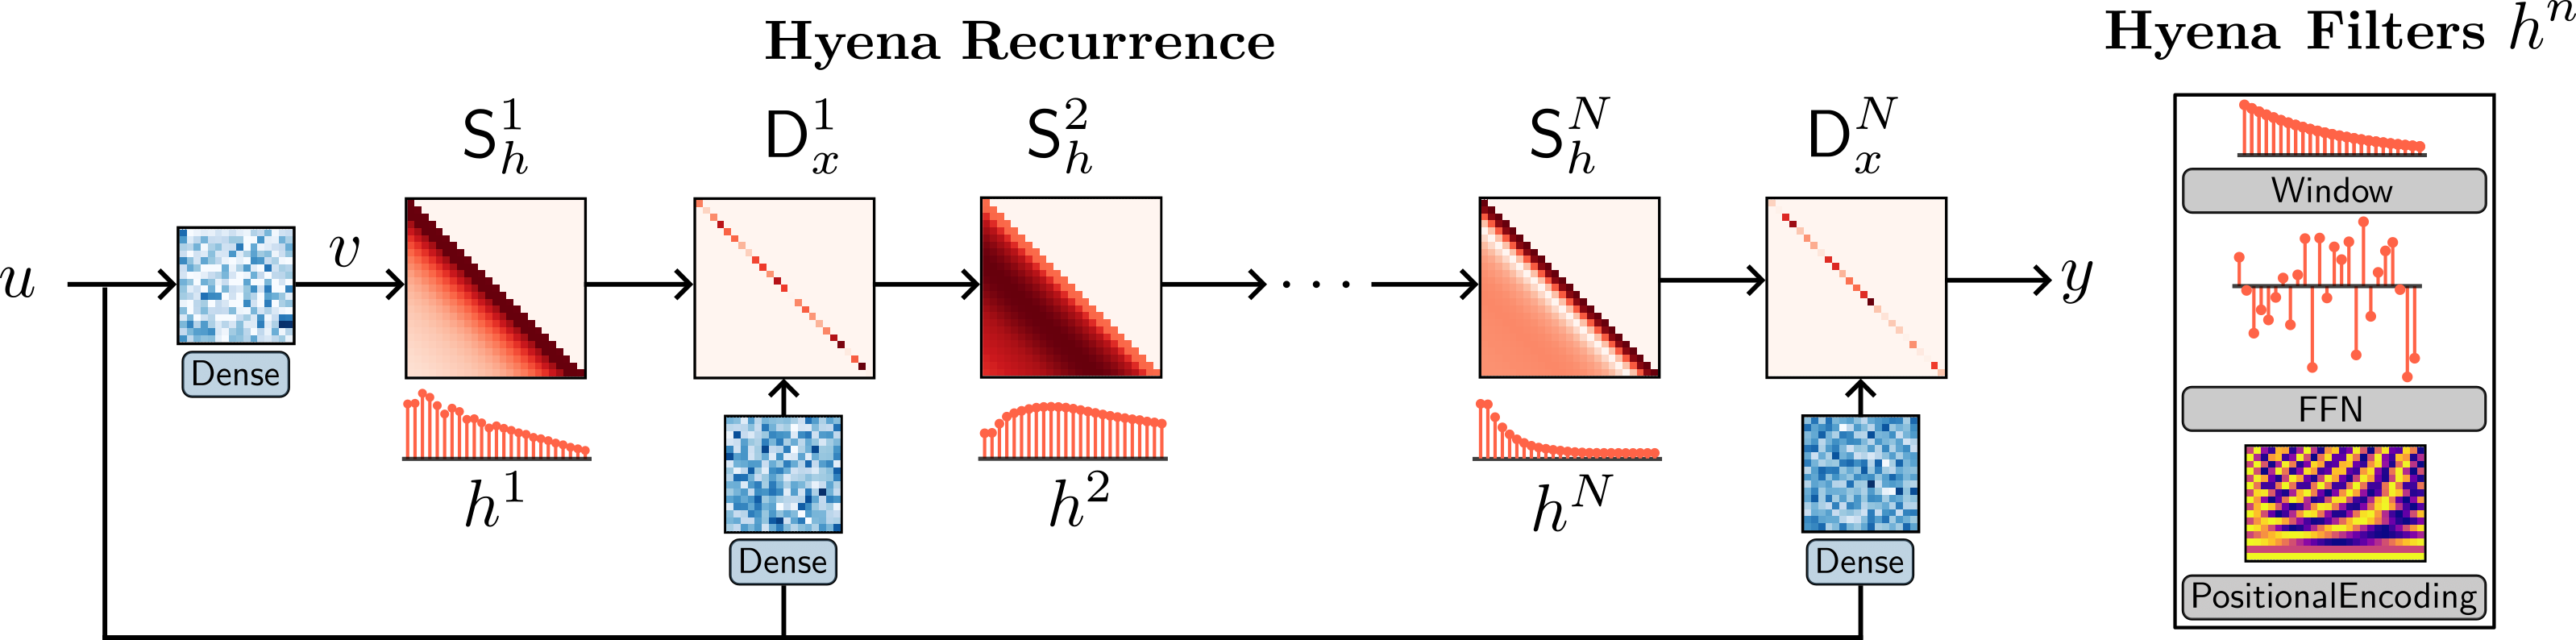
\includegraphics[width=\linewidth]{figures/hyena.png}
    \vspace{-2mm}
    \caption{The ${\sf Hyena}$ operator is defined as a recurrence of two efficient subquadratic primitives: an implicit long convolution $h$ (i.e. {\sf Hyena} filters parameterized by a feed-forward network) and multiplicative element-wise gating of the (projected) input. The depth of the recurrence specifies the size of the operator. {\sf Hyena} can equivalently be expressed as a multiplication with \textit{data-controlled} (conditioned by the input $u$) diagonal matrices $\sD_x$ and Toeplitz matrices $\sS_h$. In addition, {\sf Hyena} exhibits sublinear parameter scaling (in sequence length) and unrestricted context, similar to attention, while having lower time complexity.}
    \label{arch}
\end{figure*}
%

{\centering
\textit{Are there subquadratic operators that can match the quality of attention at scale?}\par}

\vspace{0.5cm}
% 

We obtain a positive answer based on a composition of efficient subquadratic primitives, such as \textit{element-wise multiplication} (gating) and \textit{long convolutions} i.e., convolutions with filter sizes as long as the input. We rely on a set of targeted reasoning tasks, grounded in recent work on \textit{mechanistic interpretability} \citep{elhage2021mathematical,power2022grokking,olsson2022context,zhang2022unveiling} such as recall and induction, to distill three properties of attention correlated with its performance and the quality gap with existing subquadratic approaches: 
%
\begin{itemize}[leftmargin=0.1in]
    \item[$a.$] \textbf{Data control:} Attention implements an expressive \textit{data-controlled} \citep{massaroli2020dissecting} linear operator\footnote{Self-attention can be expressed as $y = \sA(k, q) v$ where $\sA$ is the \textit{attention matrix} conditioned by linear projections $k, q$ of the input and multiplied by $v$, another projection.}, encoding an entire family of linear functions in a single block.
    \item[$b.$] \textbf{Sublinear parameter scaling:} Parameter counts of attention layers are decoupled from sequence length, allowing Transformers to allocate more parameters elsewhere e.g., the \textit{feed-forward neural networks} ({$\sf FFN$s}) between attention layers.
    \item[$c.$] \textbf{Unrestricted context:} For a given input, attention has an unrestricted context i.e., it can approximate dependencies between any two inputs, without arbitrary restrictions such as locality (except in cases using masking such as autoregressive models).
\end{itemize}
%
\paragraph{The ${\sf Hyena}$ hierarchy}
%
Guided by these findings, we introduce the ${\sf Hyena}$ hierarchy, an operator defined by a recurrence of two efficient subquadratic primitives: \textbf{a long convolution and element-wise multiplicative gating} (see Figure \ref{arch}). A specified depth (i.e., number of steps) of the recurrence controls the size of the operator. For short recurrences, existing models are recovered as special cases \citep{mehta2022long,dao2022hungry}. By mapping each step in the ${\sf Hyena}$ recurrence to its corresponding matrix form, we reveal ${\sf Hyena}$ operators to be equivalently defined as a decomposition of a \textit{data-controlled} matrix i.e., a matrix whose entries are functions of the input. Furthermore, we show how ${\sf Hyena}$ operators can be evaluated efficiently without materializing the full matrix, by leveraging fast convolution algorithms \citep{selesnick2017fast}. Empirically, ${\sf Hyena}$ operators are able to significantly shrink the quality gap with attention at scale, reaching similar perplexity and downstream performance with a smaller computational budget (Section \ref{res:lm}) and \textbf{without hybridization} of attention.
%

\paragraph{Narrowing the capabilities gap}
%
The design of {\sf Hyena} is motivated by a quality gap between standard dense attention and alternative subquadratic operators, which we identify by focusing on reasoning tasks correlated with language modeling performance at scale. We extend the suite of basic mechanistic interpretability benchmarks (\textit{induction} and \textit{recall}) with additional tasks that probe how quickly model performance degrades when task complexity increases (e.g. vocabulary size grows). In addition, we investigate the optimal parameterization of long convolutions in ${\sf Hyena}$. In the most challenging settings with hundreds of thousands of tokens, our implicit parameterization scheme improves over other operators leveraging state spaces \citep{gu2021efficiently}, frequency-domain parametrizations \citep{li2020fourier}, or standard convolutions by over $50\%$ accuracy.
%
\paragraph{Scaling in language and vision}
%
Next, we aim to verify whether rankings in our reasoning benchmark suite are predictive of quality at scale. We test ${\sf Hyena}$ on autoregressive language modeling at the sub-billion parameter scale, setting a new state-of-the-art for dense-attention-free architectures in standard datasets ({\sc WikiText103} and {\sc The Pile}) and matching Transformer quality. On the {\sc The Pile} at the $335$M parameter scale, we match Transformer perplexity with a $20\%$ reduction in the total count of \textit{floating point operations} (FLOPs). As an extension, we investigate the generality of ${\sf Hyena}$ operators by testing on large-scale image recognition, replacing attention in the Vision Transformer (ViT) \citep{dosovitskiy2020image}. In image classification, ${\sf Hyena}$ is able to match attention in accuracy when training on ImageNet-1k from scratch.
%
\paragraph{Toward much longer context}
%
Finally, we benchmark the efficiency of ${\sf Hyena}$ on long sequences. We measure $5$x speedups over dense self-attention at length $8192$ -- $2$x over highly optimized FlashAttention\footnote{FlashAttention is already 2-4x faster than a standard attention implementation in PyTorch.} \citep{dao2022flashattention} -- and $100$x speedup over FlashAttention at sequence lengths of $64$k, where standard attention implementation in PyTorch runs out of memory. 
\section{Prior Approaches}
Prior approaches to language model alignment involve directly optimizing the logits produced by the language modelling head to increase the likelihood of producing preferable responses while decreasing the likelihood of undesirable responses. %This is often realized through RLHF or contrastive methods which are outlined below.

\subsection{Reinforcement Learning from Human Feedback (RLHF)}
Reinforcement Learning from Human Feedback seeks to learn a reward model from human feedback on completions generated by a language model which can be used to align an LM with human preferences. A typical RLHF pipeline consists of 3 steps: (1) supervised fine-tuning, (2) preference sampling and reward modelling, and (3) RL fine-tuning.

\textbf{Supervised Fine-Tuning\ } The first step of a standard RLHF pipeline is fine-tuning a pre-trained LM on high quality data for downstream tasks to obtain a model $\pi^\text{SFT}$.

\textbf{Reward Modelling\ } Next, the SFT model is prompted with input tokens $x$ to produce completions $y$. These answers are then rated by human labelers which rate the answers based on one or more criteria. A reward model $r_\phi(x,y)$ is then trained to estimate the scores assigned by human labelers using maximum likelihood estimation.

\textbf{RL Fine-Tuning\ } During the RL phase the learned reward function is used to provide feedback to the language model using the following optimization problem
\begin{equation} \label{eq:rl-objective}
    \underset{\pi_\theta}{\max}\, \mathbb{E}_{x \sim \mathcal{D},y \sim \pi_\theta(y|x)}
    \left[ r_\phi(x,y) \right]
    - \beta D_{\text{KL}}\left[ \pi_\theta(y|x)||\pi_\text{ref}(y|x) \right]
\end{equation}
where $\beta$ controls the deviation from the base reference policy $\pi_{\text{ref}}$, which is typically initialized from $\pi^\text{SFT}$. Due to the non-differentiable nature of language generation this objective must be optimized using a reinforcement learning algorithm such as PPO \cite{schulman2017proximal}.

\subsection{Direct Preference Optimization (DPO)}
Direct Preference Optimization was introduced as a reparameterization of RLHF which eliminates both the sampling stage and the reward modelling stages and reformulates alignment procedure as a loss function which can be optimized directly on a dataset of pairs of preferred and dispreferred completions to given prompts. This allows DPO to stably and efficiently converge on an optimal policy using what is effectively a classification loss over positive and negative pairs.

Given a dataset $\{(x,y_w,y_l)\}$ where $x$ is the prompt and $y_w,y_l$ are the preferred and dispreferred completions, we introduce the following loss function:
%the following loss function is formulated:
\begin{equation}
    \mathcal{L}_\text{DPO}(x,y_w,y_l)=
    -\log\sigma
    \left(
        \beta\log \frac{\pi_\theta(y_w|x)}{\pi_\text{ref}(y_w|x)} -
        \beta\log \frac{\pi_\theta(y_l|x)}{\pi_\text{ref}(y_l|x)}
    \right)
    \label{eq:dpo}
\end{equation}
where $\pi_\theta(y_*|x)$ and $\pi_\text{ref}(y_*|x)$ are the probabilities of completions $y_*$ for prompt $x$ given by the policy model and reference models respectively, and the $\beta$ parameter controls the deviation from the reference policy.

There also exists an augmentation of DPO namely Conservative DPO (cDPO) \cite{cdpo} which is designed to be more robust to noisy labels through the introduction of label smoothing parameter $\epsilon$. The objective function for cDPO is given by:% the following formula:
\begin{equation}
    \mathcal{L}_\text{cDPO}(x,y_w,y_l)=
    (1-\epsilon) \mathcal{L}_\text{DPO}(x,y_w,y_l) +
    \epsilon\,\mathcal{L}_\text{DPO}(x,y_l,y_w)
    \label{eq:cdpo}
\end{equation}
\section{Direct Preference Heads}
The hypothesis underlying the Direct Preference Optimization framework of Rafailov et al. \cite{rafailov2023direct} is that a ``language model is secretly a reward model'' thereby making the purpose of Direct Preference Heads to exploit this and extract explicit reward signals without the need of an \emph{additional} reward model.

% Unlike other RLHF pipelines such as PPO \cite{schulman2017proximal}, these rewards are not used for RL fine-tuning. Instead, the DPH rewards are to be used to prune candidate generations sampled from the LM at inference time to select the candidate which aligns most with human preferences.

% This makes DPH an excellent choice for small language models which are (1) more lightweight -- and therefor can be efficiently used to generate multiple samples -- and, (2) are more prone to degradation when aligned using typical RL techniques \cite{bekbayev2023poison, bai2022training}.

\subsection{Reward Head}
% \begin{wrapfigure}{R}{5.5cm}
%     \centering
%     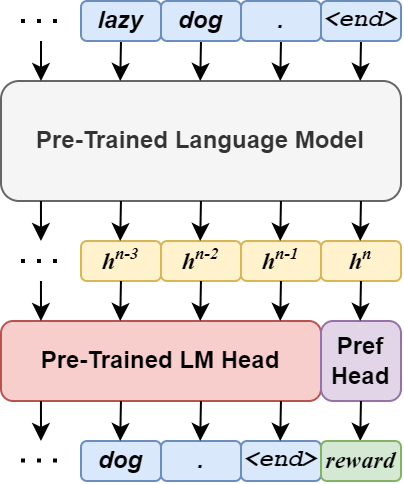
\includegraphics[width=5.5cm,trim={0 0 0 1cm}]{figures/mode_diagram.png}
%     \caption{Architecture of an LM augmented with DPH.}
% \end{wrapfigure}
To obtain the rewards from a sequence $x;y$ three components are required: an aggregated hidden state $h$ which is conditioned on the intermediate representations of the language model, a pooling function $f$ which transforms the hidden state, and a learnable vector $w_{dph}$ with the same dimension as the output of $f$. We then compute the reward $r$ as follows:
\begin{equation}
    r=f(h) \cdot w_{dph}
\end{equation}
To obtain the hidden state we take the output of the last transformer layer for the final token of the sequence, and we experiment with three choices of $f$: (1) the identity mapping following the convention established by OpenAI's GPT for sequence classification \cite{Radford2018ImprovingLU}, (2) a learnable affine projection with $\tanh$ nonlinearity following BERT's pooling function \cite{devlin2019bert}, and (3) an inverted bottleneck FFN with SwiGLU activation mirroring the FFN blocks used within the transformer backbone followed by $\tanh$ nonlinearity \cite{shazeer2020glu}.
% \begin{subequations} \label{eq:pooling_funcs}
%     \begin{alignat}{2}
%     f_{\text{GPT}}(h) &= h \\
%     f_{\text{BERT}}(h) &= \tanh{(Wx+b)} \\
%     \todo{f_{\text{SwiGLU}}(h)} &= \todo{\tanh{(W_3((W_2x + b_2)\otimes\text{SiLU}(W_1x + b_1)) + b_3)}}
%     \end{alignat}
% \end{subequations}

\subsection{Objective Function}
We formulate two novel objective functions for our method: a separable objective which maximises positive rewards and minimises negative rewards, and a contrastive objective which maximises the margin between positive and negative rewards. The loss landscapes are illustrated by Figure~\ref{fig:both_dph_loss} in the appendix.

\subsubsection{Separable DPH}
The Separable DPH loss function given by \eqref{eq:sep_dph} is a function of the preferred and dispreferred rewards $r_w,r_l$, and the label smoothing parameter $0 \leq \epsilon \leq 0.5$ which controls the reward margin.
\begin{equation} \label{eq:sep_dph}
    \mathcal{L}_\text{SepDPH}(r_w,r_l)=
    - \left[ (1-\epsilon) \log \sigma(r_w) + \epsilon\, \log \sigma(-r_w) \right]
    - \left[ \epsilon\, \log \sigma(r_l) + (1-\epsilon) \log \sigma(-r_l) \right]
\end{equation}

\begin{theorem} \label{thrm:sep_dph_convergence}
For all $\epsilon \in (0,0.5]$ the objective function $\mathcal{L}_\text{SepDPH}$ is convex and will optimize the policy $\pi_\theta$ such that the preferred rewards $r_w$ produced by the preference head converge towards $\log\tfrac{1-\epsilon}{\epsilon}$ and the dispreferred rewards $r_l$ converge to $\log\tfrac{\epsilon}{1-\epsilon}$. %\todo{When $\epsilon=0$ the objective function will never converge and gradients $\nabla_\theta \mathcal{L}_\text{SepDPH}$ will never be zero.}
\end{theorem}

This can be proven by observing the first and second partial derivatives of the loss function with respect to the rewards. The first partial derivative is equal to zero at the points $r_w=log\tfrac{1-\epsilon}{\epsilon}$ and $r_l=\log\tfrac{\epsilon}{1-\epsilon}$ respectively, and the second partial derivative is strictly positive for all values of $r_w,r_l$. A full proof is included in Appendix~\ref{sec:sep_dph_proof}.

\subsubsection{Contrastive DPH}
Like Separable DPH, the loss function for Contrastive DPH given by \eqref{eq:con_dph} is function of the preferred and dispreferred rewards $r_w,r_l$ and the label smoothing parameter $0 \leq \epsilon \leq 0.5$. This version of the loss function optimizes the \textit{relative} margin between the rewards rather than optimizing the \textit{absolute} positive and negative rewards as in Separable DPH.
\begin{equation}
    \mathcal{L}_\text{ConDPH}(r_w,r_l)=
    - (1-\epsilon) \log\sigma(r_w-r_l)
    -  \epsilon\, \log\sigma(r_l-r_w)
    \label{eq:con_dph}
\end{equation}

% \vspace{3pt}

\begin{theorem} \label{thrm:con_dph_convergence}
For all $\epsilon \in (0,0.5]$ the objective function $\mathcal{L}_\text{ConDPH}$ is convex and will optimize the policy $\pi_\theta$ such that the difference between preferred rewards $r_w$ and dispreferred rewards $r_l$ produced by the preference head will converge to a fixed margin, given by $r_{\Delta}=r_w-r_l=\log\tfrac{1-\epsilon}{\epsilon}$. %\todo{When $\epsilon=0$ the objective function will never converge and gradients $\nabla_\theta \mathcal{L}_\text{ConDPH}$ will never be zero.}
\end{theorem}

This can be proven by reparameterising the loss function such that $r_{\Delta}=r_w-r_l$ and by then considering the first and second partial derivatives with respect to this reward margin. It can be observed that the first partial derivative is equal to zero when $r_{\Delta}=\log\tfrac{1-\epsilon}{\epsilon}$, and the second partial derivative is strictly positive for all values of $r_{\Delta}$. A full proof is included in Appendix~\ref{sec:con_dph_proof}.

\subsubsection{Relation to cDPO}
The properties of both Contrastive DPH and Seperable DPH show a strong relationship with Conservative DPO: SepDPH will converge to optimal \textit{fixed reward margins} above zero for $r_w$ and below zero for $r_l$; ConDPH will converge to optimal \textit{fixed reward margins} between $r_w$ and $r_l$, and cDPO will converge to a \textit{fixed delta from the reference model} \cite{cdpo}. Like Conservative DPO, this makes both Seperable DPH and Contrastive DPH robust to preference label noise and makes training more stable than naive maximum likelihood estimation without label-smoothing.

% This establishes a strong relationship between the \textit{Contrastive DPH objective} and \textit{Conservative DPO} when label smoothing is employed, since ConDPH will converge to an optimal \textit{fixed reward margin} while cDPO will converge to a \textit{fixed delta from the reference model}. Like cDPO, this makes Contrastive DPH robust to preference label noise and will likely make training more stable \cite{cdpo}.

\subsection{Novelty over Traditional Reward Modelling}
Although similar to the reward modelling phase of an RLHF pipeline, DPH has some distinct differences which set it apart. DPH does not require an SFT sampling and human labelling stage meaning it can take advantage of pre-constructed preference datasets such as those used for DPO. Typical RLHF also requires multiple models -- a reward model, a reference model and a policy model -- while DPH requires only a single model to produce both responses and rewards. Unlike other RLHF pipelines such as PPO \cite{schulman2017proximal}, the rewards produced by DPH are not used for RL fine-tuning; instead, the DPH rewards are to be used to prune candidate generations sampled from the LM at inference time to select the candidate which aligns most with human preferences. This makes DPH an excellent choice for small language models which are (1) more lightweight -- and therefore can be efficiently used to generate multiple samples -- and, (2) are more prone to degradation when aligned using typical RL techniques \cite{bekbayev2023poison, bai2022training}.
\section{Experimental Setup and Data} \label{sec:methodology}

\subsection{Datasets}
We make use of a variety of datasets for fine-tuning and evaluation which are outlined below. The specific prompt templates used for fine-tuning and evaluation are described in Appendix~\ref{sec:datasets_cont}.

\textbf{Natural Language Understanding (NLU)\ }
For general NLU we make use of the standard \textbf{GLUE} benchmark \cite{wang2019glue}. The overall score for GLUE is computed by the macro-average of unweighted metric averages for all 9 tasks, however we also include a secondary score which does not included the `problematic' WNLI task following the evaluation used for BERT \cite{devlin2019bert}. We opted to omit WNLI during fine-tuning due to the low sample size. %, overlap of sentences in the training and validation splits, and different label distribution in the test set.

\textbf{Commonsense Reasoning\ }
In accordance with the \textbf{GPT4All} \cite{gpt4all} evaluation suite, we use the following datasets to evaluate commonsense reasoning abilities:
\textbf{HellaSwag} \cite{zellers2019hellaswag},
\textbf{OpenBookQA} \cite{mihaylov2018suit},
\textbf{WinoGrande} \cite{DBLP:journals/corr/abs-1907-10641},
\textbf{ARC} \cite{clark2018think},
\textbf{BoolQ} \cite{clark2019boolq},
and \textbf{PIQA} \cite{bisk2019piqa}.
% \textbf{HellaSwag} \cite{zellers2019hellaswag} -- an adversarially constructed sequence completion task,
% \textbf{OpenBookQA} \cite{mihaylov2018suit} -- a commonsense multiple-choice task,
% \textbf{WinoGrande} \cite{DBLP:journals/corr/abs-1907-10641} -- a fill-in-a-blank task with binary options,
% \textbf{ARC} \cite{clark2018think} -- a collection of multiple-choice grade-school science questions,
% \textbf{BoolQ} \cite{clark2019boolq} -- an open-book yes/no QA task, and
% \textbf{PIQA} \cite{bisk2019piqa} -- a QA task focused on reasoning over physical actions.

% \todo{These tasks are included in the fine-tuning and alignment mixes used to train our models. We use the macro-average of task scores as an indicator of average commonsense reasoning ability, where we use specific validation or test split used by the LM Evaluation Harness \cite{eval-harness} for consistency with other evaluations.}

\textbf{Reading Comprehension\ }
To evaluate reading comprehension abilities we use the \textbf{RACE} dataset \cite{lai2017race}, a multiple-choice task which requires reasoning over provided passages.

% \todo{We include both these tasks in our fine-tuning and alignment mixes, but opt to not include SQuAD as part of our model evaluation results; this is due to the need to reformulate SQuAD as a generative task for causal LMs which introduces a multitude of sampling and generation hyperparameters which must be ablated over. Never-the-less we do include results of a reformulated version of SQuAD V2 which compares the log-probabilities of ground-truth answers from the validation set with `distractor' spans extracted using SpaCy; this is included purely to evaluate the performance of DPH alignment and these results should not be compared with the scores of encoder-only models.}

\textbf{Instruction Following\ }
We include the \textbf{Alpaca} \cite{alpaca}, \textbf{OpenOrca} \cite{OpenOrca}, and \textbf{UltraFeedback} \cite{cui2023ultrafeedback} datasets to train our models for instruction following.
% \textbf{Alpaca} \cite{alpaca} -- a collection of 52,000 self-instruct question-answer pairs,
% \textbf{OpenOrca} \cite{OpenOrca} -- a large dataset of augmented question-answer pairs from the FLAN Collection \cite{longpre2023flan}, and
% \textbf{UltraFeedback} \cite{cui2023ultrafeedback} -- a large scale preference dataset generated from a variety of LLMs.
We make use of OpenOrca and a cleaned version of \href{https://huggingface.co/datasets/yahma/alpaca-cleaned}{Alpaca} for SFT, and binarized versions of \href{https://huggingface.co/datasets/Intel/orca_dpo_pairs}{OpenOrca} and \href{https://huggingface.co/datasets/argilla/ultrafeedback-binarized-preferences-cleaned}{UltraFeedback} for alignment.

\textbf{Auxiliary Datasets\ }
% We also make use of auxiliary train split from \textbf{MMLU} \cite{hendrycks2021measuring} to provide additional multiple-choice training data, but opt not to evaluate our models on this dataset due to requiring highly domain-specific knowledge. Additionally, we include \textbf{SQuAD V2} \cite{rajpurkar-etal-2018-know,rajpurkar-etal-2016-squad}, \textbf{Tiny Stories} \cite{eldan2023tinystories}, \textbf{CNN-Dailymail} \cite{nallapati2016abstractive} and \textbf{CoQA} \cite{reddy2019coqa} to provide signals for a wider range of tasks during SFT.
To provide additional training data for SFT we include the \textbf{MMLU} \cite{hendrycks2021measuring}, \textbf{SQuAD V2} \cite{rajpurkar-etal-2018-know,rajpurkar-etal-2016-squad}, \textbf{Tiny Stories} \cite{eldan2023tinystories}, \textbf{CNN-Dailymail} \cite{nallapati2016abstractive} and \textbf{CoQA} \cite{reddy2019coqa} training splits. For alignment we only include MMLU and SQuAD V2.

\subsection{Prompts and Sampling}
\textbf{Prompts\ } We make use of the ChatML prompt templating scheme \cite{chatml} with handcrafted \texttt{system}, \texttt{user} and \texttt{assistant} prompts specific to each task. During fine-tuning we mask out the loss for all tokens of the prompt and condition the model on the content of \texttt{assistant} messages including the final \texttt{<|im\_end|>} token. During evaluation we select the highest scoring answer using the average log-probabilities of the tokens in the final \texttt{assistant} message, or compute the reward scores on the final \texttt{<|im\_end|>} token when evaluating with DPH.

\textbf{SFT Sampling\ } \label{sec:sft-sampling} When sampling from the datasets for SFT we randomly shuffle each dataset and uniformly interleave samples from all tasks in the mix. To control the weighting of samples from each task we fill the context window with $n$ consecutive samples from the same task before sampling from a different task, where $n$ is chosen to be 5 in our experiments. To maximise compute utilisation and minimize unused portions of the context window we make us of Transformer-XL \cite{dai2019transformerxl} style training with a context window size of 2048 tokens and a recurrent memory size of 2048 tokens.

\textbf{DPH Sampling\ } \label{sec:dph-sampling} When sampling from datasets for DPH alignment we switch from the Transformer-XL style pipeline to typical SFT training, opting to only include single samples in the context window padded to a fixed maximum length. As some of the datasets we use for DPH are intended for SFT rather than alignment (namely GLUE, GPT4All, RACE, MMLU and SQuAD) we synthesise preference pairs where the `correct' answer is used as the preferred completion and we uniformly sample an `incorrect' answer from the available choices for the dispreferred completion. This is trivial for most datasets, however we use a special process for the SQuAD V2 dataset; for answerable questions we use ``unanswerable'' as the dispreferred completion, and for unanswerable questions we use SpaCy to randomly sample a noun span from the context to use as the dispreferred completion.

\subsection{Regularization} \label{sec:regularization}
The hidden states $h$ used to compute the reward scores are likely sub-optimal for computing rewards when initialising $\pi_\theta$ from $\pi^{\text{SFT}}$. As such, it may be desirable to fine-tune some or all parameters in the language model to learn better reward signals. This necessitates the use of regularization to prevent degradation of the models generative capabilities while learning to predict rewards.

\textbf{Prior Regularization\ }
Typical parameter regularization strategies such as weight decay make the assumption that parameters $\theta$ follow a zero-mean Normal distribution $p(\theta) \sim \mathcal{N}(0,\tfrac{1}{\beta}\text{I})$ leading to an auxiliary loss term $\tfrac{\beta}{2}||\theta||^2_2$. However, when performing transfer-learning or fine-tuning on a pre-trained model this assumption can be harmful and aid in catastrophic forgetting of the model's previously learnt abilities.

An alternative regularization scheme is Prior Regularization \cite{CHELBA2006382, daumé2009frustratingly, grachten2019strategies} which instead makes the assumption that the fine-tuned parameters are normally distributed around the original parameters $\theta_{\text{ref}}$, that is $\theta \sim \mathcal{N}(\theta_{\text{ref}},\tfrac{1}{\beta}\text{I})$, leading to the auxiliary loss term $\tfrac{\beta}{2}||\theta-\theta_{\text{ref}}||^2_2$.

We employ Prior Regularization to limit the divergence of $\pi_\theta$ from $\pi^{\text{SFT}}$ while still facilitating the learning of improved hidden state representations for the Direct Preference Head. Pseudocode for optimizer based decoupled prior regularization is included in Appendix~\ref{sec:decoupled-pr}.

% \paragraph{KL Divergence Regularization}
% Utilising KL Divergence as means to prevent a policy from diverging too far from the initial parameters is popular form of regularization: In TRPO the KL term is used to constrain the optimized policy \cite{schulman2017trust}, while PPO uses the KL Divergence as a penalty in the objective function \cite{schulman2017proximal}. \todo{Following PPO, we can form an auxiliary loss penalty with the following formula
% \begin{equation}
%     L_{penalty}(x,y) =
%     \beta D_{\text{KL}}\left[ \pi_\theta(y|x)||\pi_\text{ref}(y|x) \right]
% \end{equation}
% where $\beta$ is the regularization penalty. As noted in the PPO paper, the $\beta$ parameter requires careful tuning, and varying this coefficient throughout training may be required.}

\textbf{cDPO Regularization\ }
Rather than directly employing a KL Divergence penalty similar to that used in \eqref{eq:rl-objective} we find that it is possible -- and even beneficial -- to use Conservative DPO as a means of (1) limiting the divergence of the policy model to a fixed delta from the reference model, and (2) `nudging' the model towards generating more preferable outputs which increases the chance of generating a better candidate completion at inference time with fewer sampling steps.

% \paragraph{Head Regularization}
% \todo{Although both flavors of the DPH objective include label smoothing which regularizes the confidence of reward scores, it is still possible for the a preference head optimized with Contrastive DPH loss to produce rewards in divergent manor. This is due to ConDPH loss operating on the \textit{margin} of preferred and dispreferred rewards which may not necesserily be centered around zero. This can be prevented in two ways, by constraining the head weights $w_{dph}$ using weight decay or by applying a penalty to the rewards as they diverge from zero.}

\subsection{Training Pipeline}
We progressively fine-tune the models in 3 stages: vocab extension, supervised fine-tuning, and DPH alignment. The details of the pre-trained model are included in Appendix~\ref{sec:pretrained-model}.

\textbf{Vocab Extension\ } Since our model was pre-trained without a chat structure it is necessary to train the embeddings for additional \texttt{<|im\_start|>} and \texttt{<|im\_end|>} tokens: we freeze all non-embedding parameters and use the same datasets as SFT. We fine-tune the embeddings for 4096 steps with a batch size of 128, a max LR of 6e-5 which warms up over 200 steps followed by cosine decay down to zero, and clip the global gradient norm to 1.

\textbf{Supervised Fine-Tuning\ } After vocab extension we move onto the SFT step which conditions the model for NLU tasks and instruction following using the sampling and loss masking method described in section~\ref{sec:sft-sampling}. We fine-tune the model for 6144 steps with a batch size of 128, a max LR of 3e-5 which warms up over 200 steps followed by cosine decay down to zero, prior-regularization applied to all non-embedding parameters with coefficient 0.5, and clip the global gradient norm to 1.

\textbf{DPH Alignment\ } Using the sampling method described in section~\ref{sec:dph-sampling} we jointly learn DPH rewards and perform cDPO alignment. The goal here is to gently push the model towards producing preferable outputs without compromising the model's reasoning abilities, and the priority is to attain the highest validation metrics from the DPH rewards. This requires balancing the two objectives, and as such we introduce weighting parameters $\alpha_1, \alpha_2$ to our final joint objective in \eqref{eq:alignment_objective} where $\mathcal{L}_\text{DPH}$ is either $\mathcal{L}_\text{sepDPH}$ or $\mathcal{L}_\text{conDPH}$. We find $\alpha_1,\alpha_2=1$ to be a good blance between DPO and DPH in our experiments.
\begin{equation} \label{eq:alignment_objective}
    \mathcal{L}_\text{joint}(x,y_w,y_l,r_w,r_l) =
    \alpha_1 \mathcal{L}_\text{cDPO}(x,y_w,y_l) +
    \alpha_2 \mathcal{L}_\text{DPH}(r_w,r_l)
\end{equation}
We align the model for 23040 steps with a batch size of 64 pairs, a max LR of 3e-6 which warms up over 200 steps followed by cosine decay down to 3e-7, prior-regularization applied to all parameters with coefficient 0.5, and clip the global gradient norm to 1. Following the optimal DPO parameters for OpenHermes-7b-2.5 \cite{pref-tuning} we use $\beta=0.6$ and chose cDPO $\epsilon=0.25$ and DPH $\epsilon=0.1$ for regularisation. Additionally, we apply dropout with $p=0.1$ to the outputs of the pooler.

\subsection{Compute Resources}
All fine-tuning was performed using an NVIDIA A100 SXM4 80GB GPU on a compute cluster, with jobs allocated 24 cores and 160GB of memory. Each checkpoint is saved in FP16 format which consumes about 1.1GB of storage, and the datasets require minimal storage space.

For vocab extension we train for 4096 steps with an average of 7.99 seconds of compute per step which translates to about 9 hours. For supervised fine-tuning we train for 6144 steps with an average of 9.26 seconds of compute per step which translates to about 16 hours. For DPH alignment we train for 23040 steps with an average of 7.21 seconds of compute per step which translates to about 46 hours. The DPH ablations with our models use about 140 hours of compute, and the Qwen ablations use about 60 hours of compute. In total, we used approximately 270 hours of A100 compute to train our models and collect the results included in our paper. We used additional compute for preliminary tests and fixing bugs for silently failing experiments although this wasn't tracked.
\begin{table*}[ht]
    \centering
    \begin{tabular}{ccc|cc}
    \toprule
         & \multicolumn{2}{c}{AUC} & \multicolumn{2}{c}{$C_\text{max}$} \\
        $R$ & Random & Even & Random & Even\\
        \midrule
        $1$ & $0.893 \pm 0.022$ & $0.903 \pm 0.022$ & $91.43 \pm 1.60$ & $91.01 \pm 1.80$ \\ 
        \cmidrule{1-5}
        $2$ & $0.891 \pm 0.026$ & $0.890 \pm 0.025$ & $79.97 \pm 1.35$ & $73.46 \pm 1.86$ \\ 
        \cmidrule{1-5}
        $4$ & $0.869 \pm 0.022$ & $0.861 \pm 0.024$ & $61.40 \pm 1.77$ & $41.26 \pm 0.82$ \\ 
         \cmidrule{1-5}
        $8$ & $0.840 \pm 0.027$ & $0.834 \pm 0.029$ & $42.39 \pm 1.47$ & $21.51 \pm 0.51$ \\  
         \cmidrule{1-5}
        $16$ & $0.783 \pm 0.032$ & $0.754 \pm 0.032$ & $25.90 \pm 0.70$ & $10.90 \pm 0.23$ \\ 
         \cmidrule{1-5}
        $32$ & $0.682 \pm 0.022$ & $0.646 \pm 0.041$ & $13.54 \pm 0.42$ & $5.89 \pm 0.13$ \\ 
         \bottomrule
    \end{tabular}
    \caption{AUC and $C_\text{max}$ (mean and standard deviation) for \emph{Random} and \emph{Even} replacement position distribution.}
    \label{tab:uniform_vs_random_distr}
\end{table*}

Fig.~\ref{fig:auc_vs_r_main} shows how the AUC varies for increasing number of replacements $R$ made to the fuzzy trap sequences. We find that the AUC only drops slightly for smaller values of replacements $R$. For $R=4$, when $n_{\text{dup}}=10$ fuzzy trap sequences are injected, the mean AUC only drops from $0.90$ to $0.87$. Even at $R=32$, when we replace roughly one third of all tokens in the sequence, the mean AUC is $0.68$ and remains significantly higher than a single repetition $n_{\text{dup}}=1$ with a mean AUC of $0.59$. This demonstrates the mosaic memory in the target LLM, i.e. the overlapping fragments of multiple, slightly different sequences contribute to the memorization of the reference trap sequence.

\subsection{Replacement position distribution.} \label{section:spread_replacements}

We now aim to further reduce the chances of fuzzy trap sequences being removed by deduplication, and ensure that token replacements are evenly spread across the sequence. Above, we have uniformly at random sampled tokens to be replaced across fuzzy duplicates. Here, we instantiate the exact same setup, but we split the tokenized reference trap sequence using the MLM tokenizer: $T_{\text{MLM}}(X_{\text{ref}}) = \{t_1,\ldots,t_N\}$ in $R$ equally-sized chunks of size $\lceil\frac{N}{R}\rceil$. We then replace exactly one (selected uniformly at random) token for every chunk. Below we refer to this strategy as \emph{Even}, and to the previously used strategy as \emph{Random}.

We also compute the length of subsequences repeated exactly within clusters of fuzzy duplicates, simulating a sequence-level deduplication algorithm. We define $C_\text{max}$ as the maximum length (in tokens) of a substring shared by at least two fuzzy duplicate sequences within a cluster. We report the mean $C_\text{max}$ across 100 clusters used in our experiments.

Table~\ref{tab:uniform_vs_random_distr} shows that for smaller values of $R$ (up to $R=8$) the AUC for \textit{randomly} and \textit{evenly} distributed token replacements remains highly similar. For larger values of $R$ ($R \geq 16$), the impact of uniform spreading becomes more apparent, leading to a slightly lower AUC. At the same time, $C_\text{max}$ is significantly lower for the evenly distributed token replacements, with the impact more pronounced at higher values of $R$. This demonstrates how a reasonable number of token replacements ($R=4$ or $R=8$) would evade even the sequence-level deduplication with the most aggressive threshold (e.g. $50$ tokens), while retaining significant memorization.

\subsection{MIAs adapted to fuzzy trap sequences.} \label{section:adapted_mia}

So far we have used the unmodified \textit{Ratio} attack~\cite{carlini2021extracting} to infer whether the reference trap sequence has been seen by the target model. Specifically, we compute a single $\alpha(X_{\text{ref}}) = \alpha(X_1)$ for each trap sequence, and do not utilize our knowledge of the fuzzy counterparts $\{X_i \mid i=2 \ldots n_{\text{dup}}\}$. To evaluate whether this could further improve detectability, we now compute the membership score for each of the fuzzy trap sequences, i.e. $\{\alpha(X_i) \mid i=1 \ldots n_{\text{dup}}\}$, and aggregate the membership scores with aggregation function $\mathcal{A}(\cdot)$, i.e. $\alpha_{\mathcal{A}}(X_{\text{ref}}) = \mathcal{A}\left( \{\alpha(X_i) \mid i=1 \ldots n_{\text{dup}}\}\right)$. We then compute $\alpha_{\mathcal{A}}(X_{\text{ref}})$ for each reference trap sequence. We compute AUC on a balanced set of \emph{members} and \emph{non-members}, and so generate fuzzy trap sequences for all non-member sequences too. As aggregation function $\mathcal{A}$ we consider the mean, median, minimum and maximum. We report the MIA AUC for all aggregation functions, and for $R=\{2, 8, 32\}$ for models trained in the main experiment (Fig.~\ref{fig:auc_vs_r_main}). As a baseline, we also provide the previously used MIA based on the reference trap sequence $\alpha(X_{\text{ref}})$ alone.

 Table~\ref{tab:custom_MIA} shows that aggregating the membership score on all fuzzy trap sequences $\alpha_{\mathcal{A}}(X_{\text{ref}})$ does not provide substantial benefits compared to the baseline. We attribute this to the fact that all fuzzy trap sequences $X_i$ only differ from $X_{\text{ref}}$ by $R$ replacements, and therefore the target model loss computed on the reference trap sequence likely captures an aggregation across its fuzzy trap sequences already.

\begin{table*}[ht]
    \centering
    \begin{tabular}{cccc}
    \toprule
         & \multicolumn{3}{c}{AUC} \\
        Aggregation $\mathcal{A}$ & $R=2$ & $R=8$ & $R=32$ \\
        \midrule
        $\alpha(X_{\text{ref}})$ - no aggregation & $0.891 \pm 0.026$ & $0.840 \pm 0.027$ & $0.682 \pm 0.022$ \\ 
         \midrule
         \midrule
        Mean & $0.870 \pm 0.021$ & $0.828 \pm 0.029$ & $0.683 \pm 0.026$ \\ 
         \cmidrule{1-4}
        Median & $0.869 \pm 0.028$ & $0.824 \pm 0.030$ & $0.692 \pm 0.039$ \\  
         \cmidrule{1-4}
        Minimum & $0.881 \pm 0.021$ & $0.823 \pm 0.030$ & $0.624 \pm 0.040$  \\ 
         \cmidrule{1-4}
        Maximum & $0.879 \pm 0.030$ & $0.821 \pm 0.034$ & $0.679 \pm 0.041$  \\ 
         \bottomrule
    \end{tabular}
    \label{tab:custom_MIA}
    \caption{AUC (mean and standard deviation) for MIA methodologies adapted to fuzzy trap sequences.}
\end{table*}



\subsection{Ablation studies.} \label{section:ablations}

\textbf{Token replacement hyperparameters.} We here explore whether the semantic coherence of fuzzy trap sequences $X_i$ affect memorization. For this, we vary the value $k$ when sampling replacements from the top-$k$ tokens predicted by the MLM when a fixed number $R=8$ of replacements are made (see Sec.~\ref{sec:method_gen_fuzzy}). Recall that thus far we only considered $k=50$ and that for $k=|\mathcal{V}_{\text{MLM}}|$ -which is $50,000$ for RoBERTa~\cite{liu2019roberta}-, we effectively randomly sample a token from the entire MLM vocabulary $\mathcal{V}_{\text{MLM}}$. In addition to sampling uniformly from the top $k$ tokens, we also consider sampling directly from the full probability distribution predicted by the MLM (\textit{Sample directly}).

Fig.~\ref{fig:robustness}(a) shows that the AUC decreases as $k$ increases. We find $k$ and AUC to be strongly correlated with a Spearman coefficient of $-0.47$ and a p-value of \num{4e-11}, suggesting that semantic coherence is important for mosaic memorization. Further, Fig.~\ref{fig:robustness}(b) compares the AUC for $k=50$ and $k=|\mathcal{V}_{\text{MLM}}|$ for increasing values of $R$. For a smaller amount of replacements $R$, the AUC for $k=50$ and random token replacement remains very similar. For larger values of $R$ the mean estimations start to diverge, yet with no statistically significant difference.

\textbf{Impact of learning rate.} We here show, that the key outcome of our experiments - the \emph{relative} memorization of fuzzy duplicates compared to exact duplicates holds regardless of the \emph{absolute} level of memorization. At a fixed number of training steps we can control the baseline memorization with varying learning rate. So far in previous experiments, we have considered a fixed learning rate of $\num{3e-6}$. Fig.~\ref{fig:robustness} (b) shows how for increasing learning rate the AUC for fuzzy trap sequences remains consistently slightly lower than the upper bound ($n_{dup} = 10$), while remaining significantly higher than the lower bound ($n_{dup} = 1$). This suggests that fuzzy trap sequences are also memorized in lower and higher memorization regimes. 

\begin{figure*}[ht]
\centering
\subfigure{
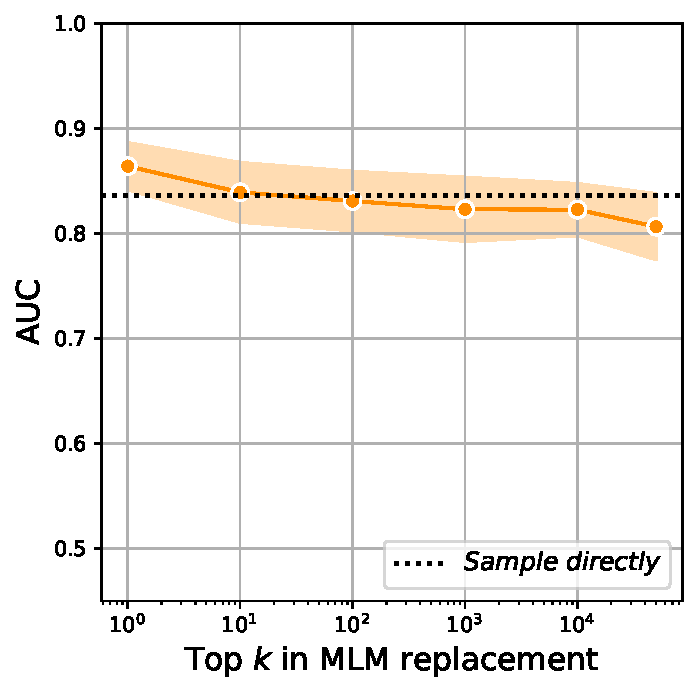
\includegraphics[width=0.3\linewidth]{figures/vary_k.pdf}
}
\subfigure{
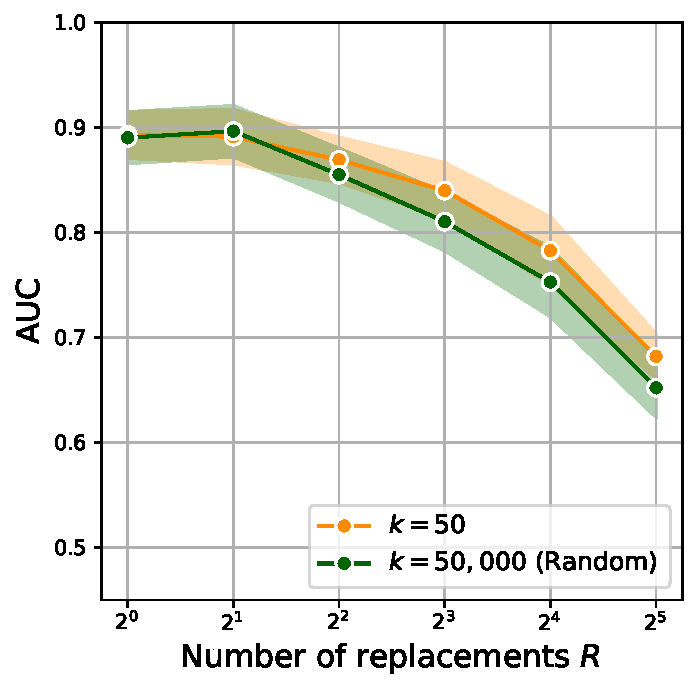
\includegraphics[width=0.3\linewidth]{figures/AUC_vs_R_both_strategies.pdf}
}
\subfigure{
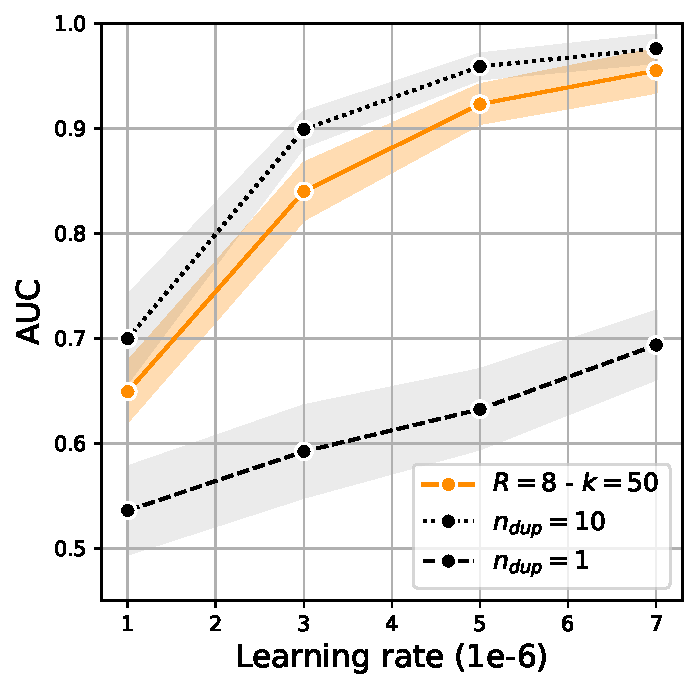
\includegraphics[width=0.3\linewidth]{figures/vary_lr.pdf}
}

    \caption{\textbf{Ablation.} MIA AUC (mean and standard deviation) for fuzzy trap sequences for (a) varying $k$ for $R=8$, (b) $k=50$ and $k=50,000$ across $R$ and (c) varying learning rate used in fine-tuning.} 
\label{fig:robustness}
\end{figure*} 

\section{Discussion}
% \subsection{Concurrent Work}
% In recent years it has become more popular to release ``uncensored'' language models, and with that there have been tools and techniques developed to detect undesirable outputs produced by these models. One such tool is Llama Guard \cite{inan2023llama}, a large language model designed to perform both prompt- and response-classification to maximise the safety of chat systems. Like DPH, Llama Guard can be used to detect and reject harmful outputs produced by a language model. However, unlike DPH, Llama Guard is an entirely separate model which must be run concurrently with chat model and therefor increases the compute and memory requirements of the combined system. % this especially contrasts with DPH being especially suited for small language models which inherently require a much smaller compute budget.

\subsection{Future Work}
As shown in the results section, DPH is capable of learning to assign higher rewards to preferred outputs and lower rewards to dispreferred outputs which implies the pooling function learns rich features with respect to prompt-completion pairs. We believe that it would be possible to also extract additional information from the output of the pooling function to detect finer grained signals such as helpfulness, humor, creativity, toxic content, etc. This can be achieved by training on a conversational dataset such Open Assistant \cite{köpf2023openassistant} which contains a variety of human-curated labels in addition to machine-generated labels produced by Detoxify \cite{Detoxify}.

% It is also worth examining how the performance of DPH scales with larger language models, and if it can be used as a post-hoc technique to provide safety guardrails for uncensored language models such as Mistral 7B and observe how it performs compared to systems such as Llama Guard while maintaining much lower compute requirements.

\subsection{Limitations}
The main benefit of DPH being its ability to perform alignment without directly effecting the model's output distribution is also its main limitation: unlike other alignment techniques which can help prevent the model generating harmful outputs, DPH is only capable of \textit{detecting} harmful outputs. Although we do include DPO alignment in our experiments to reduce the likelihood of harmful outputs, DPH does not require such model alignment to function, which shifts the responsibility of rejecting harmful outputs to the end user or service provider.

\subsection{Conclusion}
In this paper we introduced Direct Preference Heads, a novel form of language model alignment which is performed at inference time to prune candidate completions for a given prompt. Unlike other alignment techniques which coerce the model into generating human preference aligned outputs, DPH instead produces reward scores for candidate outputs without affecting the actual generation process and therefor avoids the issue of RLHF leading to degraded performance when applied to smaller language models. We formulated two loss functions for DPH and find strong connections to Conservative DPO, implying that DPH is robust to label noise and can be tuned to a specific confidence margin. Finally, we evaluated our methods on a number of NLU, commonsense reasoning and reading Comprehension tasks and found that DPH is able to consistently outperform both our SFT baseline and multiple publicly available language model checkpoints of varying size and training volume.

\subsection*{Broader Impacts}
As with all language modeling systems we cannot guarantee all responses produced by our models are factually correct nor can we guarantee that they are safe and free from harmful content. Our work focuses on creating a system that helps filter out incorrect and harmful messages by scoring candidate outputs, but as with all alignment techniques our models may be susceptible to so-called `jailbreaks' which can coerce the model into incorrectly assigning a higher score to less desirable content. To maximise safety DPH should be implemented alongside other safety guardrails such as Llama Guard \cite{inan2023llama} when used for publicly facing chat systems, and we intend for our provided model checkpoints to be used for reproduction of results and further research in the field of alignment.

\begin{ack}
% \todo{Do we need acknowledgements?}
\end{ack}

{
    \small
    \bibliographystyle{ieeenat_fullname}
    \bibliography{main}
}

%%%%%%%%%%%%%%%%%%%%%%%%%%%%%%%%%%%%%%%%%%%%%%%%%%%%%%%%%%%%

\appendix

% \section{Claimed Emergent Abilities}
% \label{app:claimed_emergent_abilities}

% We compile the models, tasks and metrics that different papers have claimed reveal emergent abilities of large language models. This list may be incomplete or inaccurate, but represents a good faith attempt to compile this information. Note: quantifying model scale when an ability emerges is complicated by the fact that different papers report model scale differently, either as (a) number of parameters \cite{brown2020language, ganguli2022predictability}, (b) effective number of parameters \cite{srivastava2022beyond} or (c) training FLOPs \cite{wei2022emergent}.

% \begin{table}[h!]
%     \centering
%     \begin{tabular}{|l|c|c|c|}
%     \hline
%         Task & Model Families & Metric & Model Scale at Emergence \\
%         \hline
%         2-Digit Addition \cite{brown2020language} & GPT-3 & Accuracy & 13B Parameters\\
%         2-Digit Subtraction \cite{brown2020language} & GPT-3 & Accuracy & 13B Parameters\\
%         3-Digit Addition \cite{brown2020language, ganguli2022predictability} & GPT-3 & Accuracy & 175B Parameters\\
%         3-Digit Subtraction \cite{brown2020language} & GPT-3 & Accuracy & 175B Parameters\\
%         MMLU \cite{ganguli2022predictability} & GPT-3, Gopher & Accuracy & 200B, 300B Parameters\\
%         Program Synthesis \cite{ganguli2022predictability} & Google Internal & \% Samples Solving Task & 200B Parameters\\
%         Figure of Speech Detection \cite{srivastava2022beyond} & ? & ? & $\sim 10^{11}$ Effective Parameters \\
%         IPA Transliterate \cite{srivastava2022beyond, wei2022emergent} & LaMDA, GPT-3 & BLEU & $\sim 10^{23}, \sim 10^{23}$ Training FLOPs\\
%         Periodic Elements \cite{srivastava2022beyond} & ? & ? & ?\\
%         Modified Arithmetic \cite{srivastava2022beyond, wei2022emergent} & GPT-3, LaMDA & Accuracy & $\sim 10^{23}, \sim 10^{24}$ Training FLOPs\\
%         Repeat Copy Logic \cite{srivastava2022beyond} & ? & ? & $10^{11}$ Effective Parameters\\
%         Word Unscrambling \cite{srivastava2022beyond, wei2022emergent} & LaMDA & Exact Match & $\sim 10^{24}$ Training FLOPs\\
%         Persian QA \cite{wei2022emergent} & PaLM & Exact Match & $\sim 10^{24}$ Training FLOPs\\
%         Truthful QA \cite{wei2022emergent} & Gopher & Accuracy & $\sim 10^{23}$ Training FLOPs\\
%         Grounded Mappings \cite{wei2022emergent} & ? & ? & ?\\
%         Multi-task NLU \cite{wei2022emergent} & ? & ? & ?\\
%         Word in context \cite{wei2022emergent} & ? & ? & $\sim 10^{24}$ Training FLOPs\\
%         \hline
%     \end{tabular}
%     \newline
%     \caption{\textbf{Tasks, model families, metrics and number of parameters for emergent abilities.}}
%     \label{tab:my_label}
% \end{table}


% \section{Exponentiated Negative Cross Entropy Lower Bounds Accuracy}
% \label{app:acc_bound}

% Consider batch size $B$ with length $L$. During training i.e. with teacher-forcing, the per-token accuracy (averaged over batch index $b$ and sequence index $l$) is defined as:
% %
% \begin{align}
%     \text{Acc} &\defeq \frac{1}{B} \sum_b \frac{1}{L} \sum_l p(t_{bl}^* | t_{b, <l}^*)\\
%     &= \frac{1}{BL} \sum_{b, l} p(t_{bl}^* | t_{b, <l}^*)
% \end{align}

% The cross entropy (commonly averaged over the batch) is defined as:
% %
% \begin{align}
%     \mathcal{L}_{CE} &\defeq -\frac{1}{B} \sum_b \log p(t_{b 1}^*, ..., t_{b L}^*)\\
%     &= -\frac{1}{B} \sum_b \log \prod_l p(t_{b l}^*| t_{b, <l}^*)\\
%     &= -\frac{1}{B} \sum_{b, l} \log p(t_{bl}^* | t_{b, <l}^*)
% \end{align}

% To make the comparison between accuracy and cross entropy a little easier, let's normalize the cross entropy by the sequence length:
% %
% \begin{align}
%     \mathcal{L}_{CE/L} &\defeq \frac{1}{L}\mathcal{L}_{CE}\\
%     &=  -\frac{1}{BL} \sum_{b, l} \log p(t_{bl}^* | t_{b, <l}^*)
% \end{align}

% Recall that Jensen's inequality tells us that for any random variable $X$, $\log \mathbb{E}[X] \geq \mathbb{E}[\log X]$. The relationship between sequence-length-normalized cross entropy and accuracy is thus:
% %
% \begin{align}
%     -\mathcal{L}_{CE/L} = \frac{1}{BL} \sum_{b, l} \log p(t_{bl}^* | t_{b <l}^*) &\leq \log \frac{1}{BL} \sum_{b, l}  p(t_{bl}^* | t_{b <l}^*) = \log \text{Acc}\\
%     \exp(- \mathcal{L}_{CE/L}) &\leq \text{Acc}
% \end{align}

% Consequently, we see that driving the cross entropy loss to $0$ necessarily drives the accuracy to $1$.

% TODO: Can we use the second moment method to derive bounds on how (un)likely a subset of tokens are to deviate from the mean?


\section{Approximate Behavior of Metrics on Sequential Data}
\label{app:metric_scaling}

How do different metrics behave when used to measure autoregressive model outputs? Precisely answering this question is tricky and possibly analytically unsolvable, so we provide an approximate answer here.

Notationally, we consider $N$ test data of length $L$ (here, length is measured in tokens) with targets denoted $t_n \defeq (t_{n1}, t_{n2}, ... t_{nL})$, the autoregressive model has a true-but-unknown per-token error probability of $\epsilon \in [0, 1]$ and the model outputs prediction $\hat{t}_n \defeq (\hat{t}_{n1}, \hat{t}_{n2}, ... \hat{t}_{nL})$. This assumes that the model's per-token error probability is constant, which is empirically false, but modeling the complex dependencies of errors is beyond our scope.

\subsection{Per-Token Error Probability is Resolution-Limited}
\label{app:metric_scaling:resolution_limited}

Note that because we have $N$ test data, each of length $L$, our resolution for viewing the per-token error probability $\epsilon$ is limited by $1/NL$. 
Here, resolution refers to ``the smallest interval measurable by a scientific instrument; the resolving power."
To explain what resolution means via an example, suppose one wants to measure a coin's probability of yielding heads.
After a single coin flip, only two outcomes are possible (H, T), so the resolution-limited probability of heads is either $0$ or $1$.
After two coin flips, four outcomes are possible (HH, HT, TH, TT), so the resolution-limited probability of heads is now one of $0, 0.5, 1$.
After $F$ coin flips, we can only resolve the coin's probability of yielding heads up to $1/F$.
Consequently, we introduce a resolution-limited notation:
%
\begin{equation}
    \nint{a}_b \defeq \text{$a$ rounded to the nearest integer multiple of $1/b$}
\end{equation}

\subsection{Token Edit Distance}
\label{app:metric_scaling:token_edit_distance}

We first consider an adaptation of the Levenshtein (string edit) distance for models that function on tokens rather than characters, an adaptation we term the \textit{token edit distance}. The token edit distance between two token sequences $t_n, \hat{t_n}$ is defined as the integer number of additions, deletions or substitutions necessary to transform $t_n$ into $\hat{t}_n$ (or vice versa).

\begin{align}
    \text{Token Edit Distance}(t_n, \hat{t}_n)  &\defeq \text{Num Substitutions} + \text{Num. Additions} + \text{Num. Deletions}\\
    &= \sum_{\ell =1}^L \mathbb{I}[t_{n\ell} \neq \hat{t}_{n\ell}] + \text{Num. Additions} + \text{Num. Deletions}\\
    &\geq \sum_{\ell =1}^L \mathbb{I}[t_{n\ell} \neq \hat{t}_{n\ell}]
\end{align}

The expected token edit distance is therefore:

\begin{align}
    \mathbb{E}[\text{Token Edit Distance}(t_n, \hat{t}_n)] &\geq \mathbb{E}[\sum_{\ell =1}^L \mathbb{I}[t_{n\ell} \neq \hat{t}_{n\ell}]]\\
    &= \sum_{\ell =1}^L p(t_{n\ell} \neq \hat{t}_{n\ell})\\
    &\approx L (1 - \epsilon)
\end{align}

The resolution-limited expected token edit distance is therefore:

\begin{equation}
    \nint{\mathbb{E}[\text{Token Edit Distance}(t_n, \hat{t}_n)]}_{NL} \geq L \Big(1 - \nint{\epsilon}_{NL} \Big)
\end{equation}

From this, we see that the expected token edit distance scales approximately linearly with the resolution-limited per-token probability. The real rate is slightly higher than linear because additions and deletions contribute an additional non-negative cost, but modeling this requires a model of how likely the model is to overproduce or underproduce tokens, which is something we do not currently possess.

\subsection{Accuracy}
\label{app:metric_scaling:accuracy}

\begin{align}
    \text{Accuracy}(t_n, \hat{t}_n) &\defeq \mathbb{I}[\text{No additions}] \, \mathbb{I}[\text{No deletions}] \, \prod_{l=1}^L \mathbb{I}[t_{nl} = \hat{t}_{nl}]\\
    &\approx \prod_{l=1}^L \mathbb{I}[t_{nl} = \hat{t}_{nl}]
\end{align}

As with the Token Edit Distance (App. \ref{app:metric_scaling:accuracy}), we ignore how likely the language model is to overproduce or underproduce tokens because we do not have a good model of this process. Continuing along,

\begin{align}
    \mathbb{E}[\log \text{Accuracy}] &= \sum_l \mathbb{E}[\log \mathbb{I}[t_{nl} = \hat{t}_{nl}]]\\
    &\leq \sum_l \log \mathbb{E}[\mathbb{I}[t_{nl} = \hat{t}_{nl}]]\\
    &\approx L \log (1- \epsilon)
    % \exp(\mathbb{E}[\log \text{Accuracy}]) &= \exp (\sum_l \mathbb{E}[\log \mathbb{I}(t_{nl}, \hat{t}_{nl})])\\
    % &=
\end{align}

Taking an approximation that would make most mathematicians cry:

\begin{align}
    \mathbb{E}[\text{Accuracy}] &\approx \exp(\mathbb{E}[\log \text{Accuracy}])\\
    &= (1 - \epsilon)^L\\
\end{align}

This reveals that accuracy \textbf{approximately} falls geometrically with target token length. The resolution-limited expected accuracy is therefore:

\begin{equation}
    \nint{\mathbb{E}[\text{Accuracy}]}_{NL} = \nint{(1 - \epsilon)^L}_{NL}
\end{equation}

From this we can see that choosing a nonlinear metric like Accuracy is affected significantly more by limited resolution because Accuracy forces one to distinguish quantities that decay rapidly.

\subsection{ROUGE-L-Sum}
\label{app:metric_scaling:rougeLsum}

\begin{figure}
    \centering
    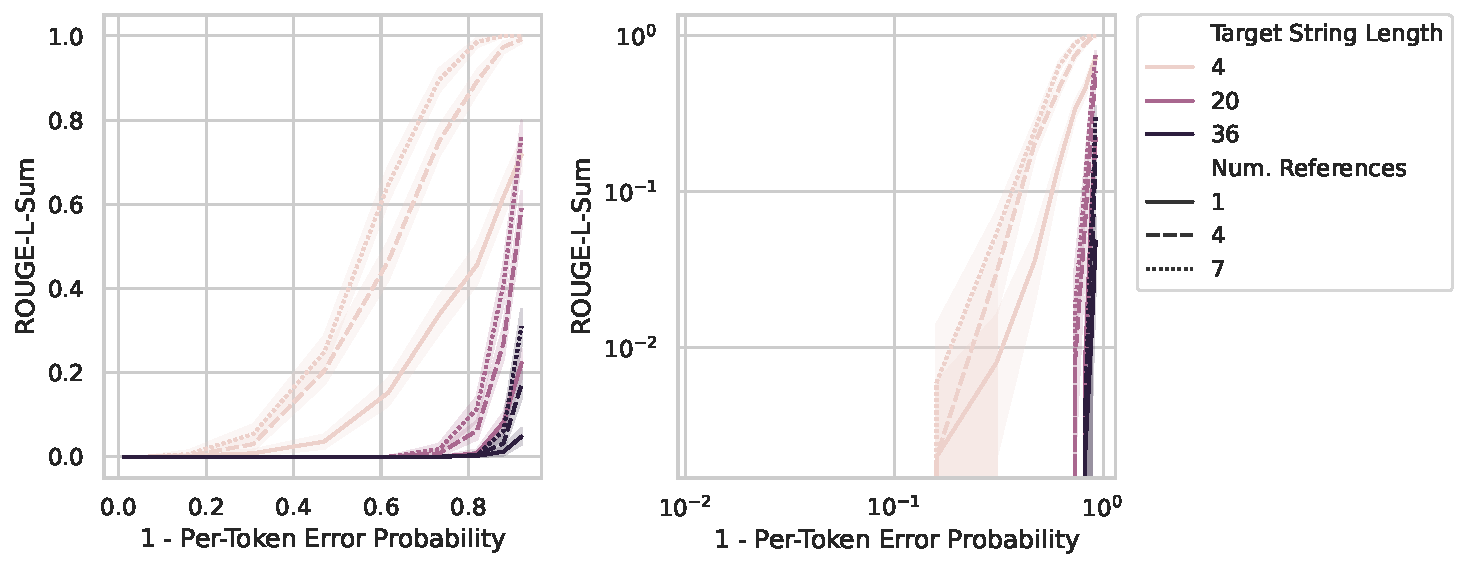
\includegraphics[width=0.95\textwidth]{figures/rouge_understanding/rougeLsum_vs_token_error_prob_scaling_simulation.pdf}
    \caption{\textbf{ROUGE-L-Sum is a sharp metric.} Simulations show that as the per-token error probability slightly increase (e.g. from 0.05 to 0.1), the ROUGE-L-Sum metric sharply falls.}
    \label{fig:app:metric_scaling:rougeLsum}
\end{figure}


Another BIG-Bench metric \cite{srivastava2022beyond} is ROUGE-L-Sum \cite{lin2004rouge}, a metric based on the longest common subsequence (LCS) between two sequences. Section 3.2 of \cite{lin2004rouge} gives the exact definition, but the key property is that ROUGE-L-Sum measures the ``union" LCS, which means ``stitching" together LCSs across the candidate and multiple references. As explained in the original paper: if the candidate sequence is $c = w_1 w_2 w_3 w_4 w_5$, and if there are two reference sequences $r_1 = w_1 w_2 w_6 w_7 w_8$ and $r_2 = w_1 w_3 w_8 w_9 w_5$, then $LCS(r_1, c) = w_1 w_2$ and $LCS(r_2, c) =w_1 w_3 w_5$, then the \textit{union} 
-LCS of $c, r_1, r_2$ is $w_1 w_2 w_3 w_5$, with length 4. Intuitively, this disproportionately benefits models with smaller error rates because their mistakes can be ``stitched" across multiple references; this is confirmed in simulation (Fig. \ref{fig:app:metric_scaling:rougeLsum}).


% \subsection{BLEU}
% \label{app:metric_scaling:bleu}


% \subsection{Emergence does not require on scaling laws: decreasing cross-entropy loss and stricter exact match is all you need }

% The goal of this section is to show that scaling laws are not necessary to create emergence and that many functional forms of the loss are valid as long as the form decreases as some other variable decreases -- say the number of parameters in the model.
% This typically holds in modern machine learning. 
% We do this by considering different functional forms of the cross entropy $CE(N)$, as a function of the number of parameters $N$, and show emergence, i.e. sharpness and unpredictability.
% We illustrate this by showing the programmer can exaggerate the sharpness (and therefore emergence) by implying increasing the exact number of tokens required to get correct in the accuracy, i.e. increasing $L$ in our notation.

% \subsubsection{Argument}

% Recall from section \ref{sec:alt_explanation} the accuracy requiring all $L$ tokens to be correct for a model of size $N$ as a function of cross-entropy $CE(N)$:

% \begin{equation*}
%     \text{Accuracy}(N) \approx p_N(\text{single token correct})^{\text{num. of tokens}} = \exp \Big(- CE(N) \Big)^L
% \end{equation*}

% We plot this equation using three functional forms for a decreasing cross-entropy loss in figure \ref{fig:decreasing_loss_leads_to_emergence_as_L_increases} for increasing values of $L$.
% These increasing values of $L$ induce a sharper -- therefore, seemingly more emergent curve when plotting the accuracy. 
% This means that if the programmer simply requires a stricter accuracy, he can make a perfectly smooth and predictable cross-entropy loss suddenly become sharp and unpredictable, i.e. ``emergent". 
% We show numerically it is independent of the functional form and instead that it only requires the cross-entropy to be decreasing and the accuracy metric to have some non-linear transformation that makes it sharper. 
% Therefore, if one had only tracked the cross-entropy loss instead, one could have had a smooth predictable curve for the models.
% This implies small-scale experimentation is still relevant, and we wish to highly that GPT-4 \cite{gpt4} small-scale experiment in conjunction with scaling loss. 
% We'd like to emphasize that changing the evaluation metric can suddenly induce emergence, and it is not an intrinsic property of the model. 

% %The goal will be to show that if $CE(N)$ decreases with different functional forms that $acc$ is emergent (either sharp or unpredictable).
% % TODO: sharp due to L
% % TODO: unpredictable due to constant and L

% \begin{figure}[htbp]
%   \centering
%   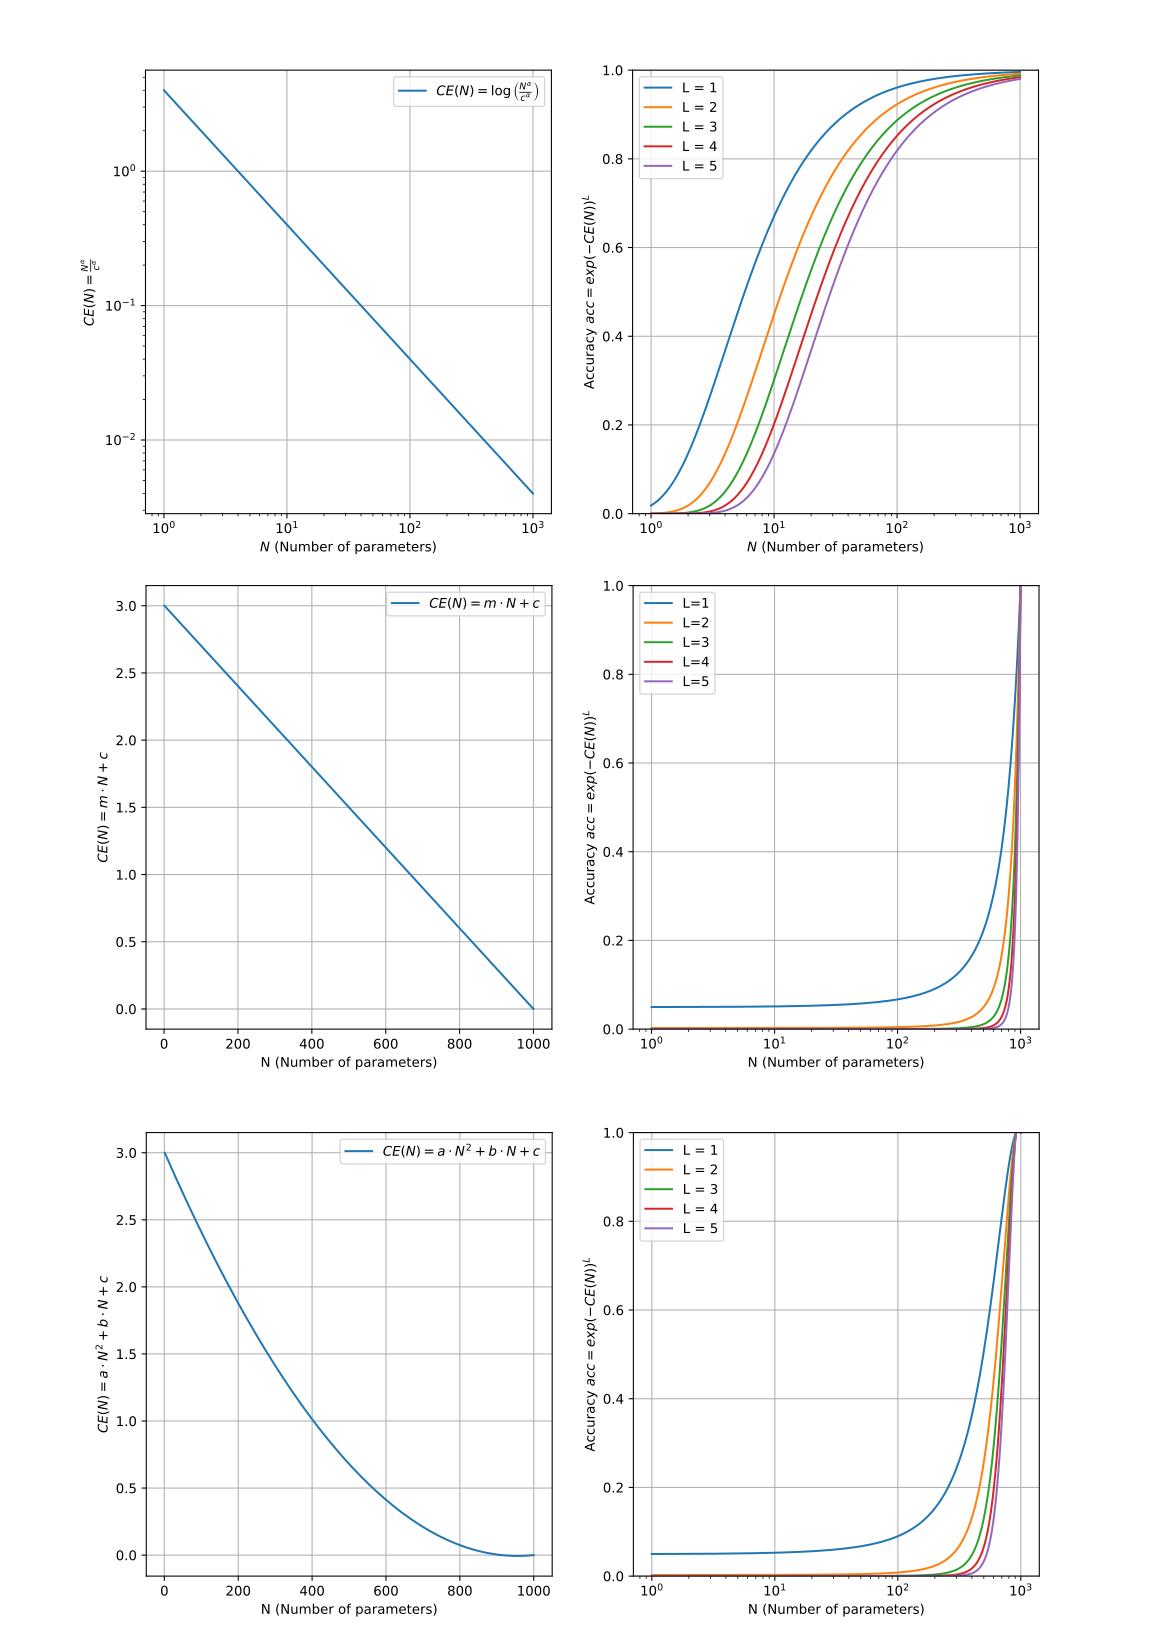
\includegraphics[width=0.8\textwidth]{figures/loss_decreasing_leads_to_emergence/decreasing_loss_leads_to_emergence_as_L_increases.png}
%   \caption{
%   \textbf{Emergence does not depend on scaling laws: any decreasing cross-entropy loss induces apparent emergence as L increases as you require more tokens to be exactly correct, i.e. L increases.}
%   The first row shows the same argument as in the main section, where a decreasing cross-entropy loss as a scaling law induces emergence as $L$ increases.
%   The second row shows the that apparent emergence is induced even when the cross-entropy loss decreases linearly.
%   The third row shows that the apparent emergence is induced when the cross-entropy loss decreases quadratically.
%   Emergence is amplified in this case especially by the increase in sharpness as more tokens are required to be correct. 
%   This means that simply changing the evaluation metric can suddenly induce emergence, and it is not an intrinsic property of the model. 
%   }
%   \label{fig:decreasing_loss_leads_to_emergence_as_L_increases}
% \end{figure}


\section{Inducing Emergent Abilities in Networks on Vision Tasks}
\label{app:sec:inducing_emergence_vision}

\subsection{Emergent Classification of MNIST Handwritten Digits by Convolutional Networks}

\begin{figure}
    \centering
    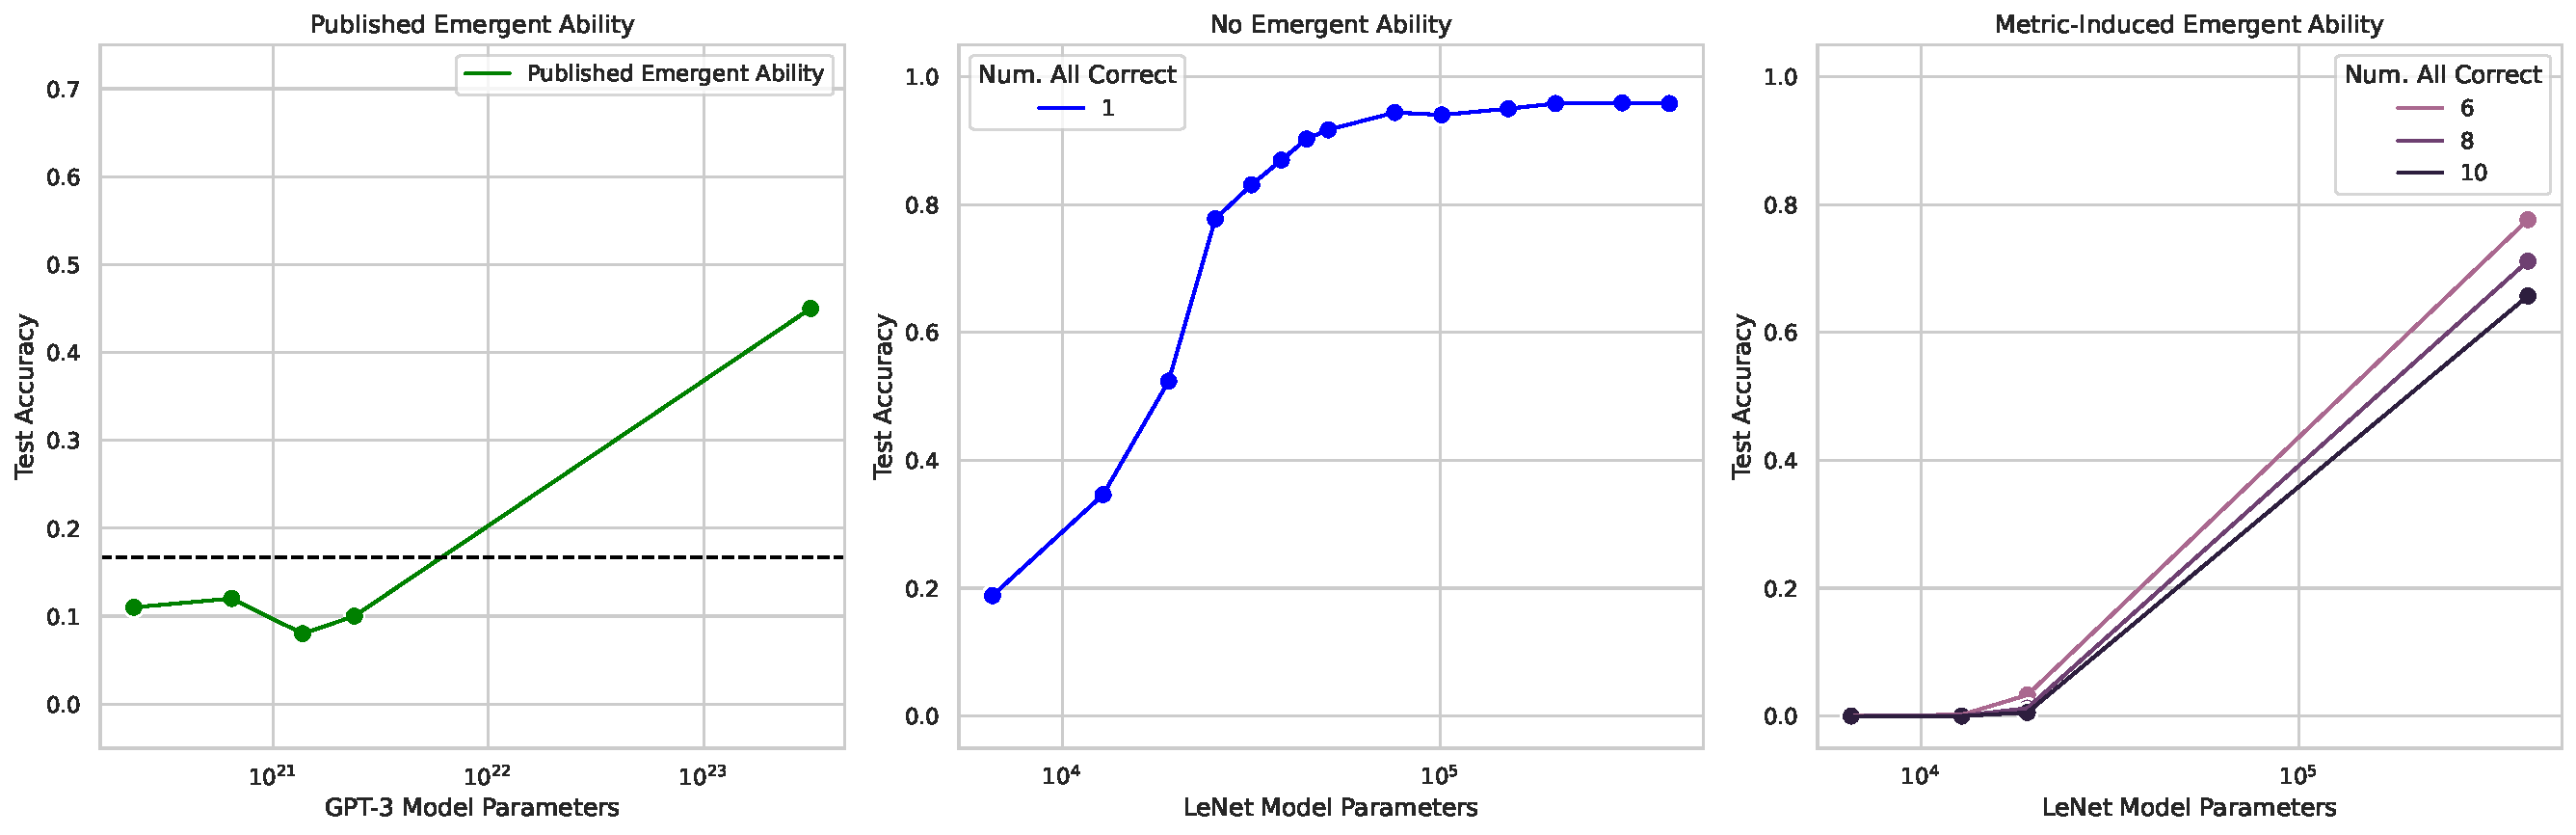
\includegraphics[width=\textwidth]{figures/vision/no_emergence_and_emergence_dataset=mnist.pdf}
    \caption{\textbf{Induced emergent MNIST classification ability in convolutional networks.} (A) A published emergent ability from the BIG-Bench Grounded Mappings task \cite{wei2022emergent}. (B) LeNet trained on MNIST \cite{lecun1998mnist} displays a predictable, commonplace sigmoidal increase in test accuracy as model parameters increase. (C) When accuracy is redefined as correctly classifying $K$ out of $K$ independent test data, this newly defined metric induces a seemingly unpredictable change.}
    \label{fig:vision_mnist}
\end{figure}

We begin by inducing an emergent classification ability in a LeNet convolutional neural network family \cite{lecun1998gradient}, trained on the MNIST handwritten digits dataset \cite{lecun1998mnist}.
This family displays smoothly increasing test accuracy as the number of parameters increase (Fig. \ref{fig:vision_mnist}B).
To emulate the accuracy metric used by emergence papers \cite{ganguli2022predictability, wei2022emergent, srivastava2022beyond}, we use \textit{subset accuracy}: 1 if the network classifies $K$ out of $K$ (independent) test data correctly, 0 otherwise.
Under this definition of accuracy, the model family displays an ``emergent" ability to correctly classify sets of MNIST digits as $K$ increases from $1$ to $5$, especially when combined with sparse sampling of model sizes (Fig. \ref{fig:vision_mnist}C).
This convolutional family's emergent classification ability qualitatively matches published emergent abilities, e.g., at the BIG-Bench Grounded Mappings task \cite{wei2022emergent} (Fig. \ref{fig:vision_mnist}A).


%%%%%%%%%%%%%%%%%%%%%%%%%%%%%%%%%%%%%%%%%%%%%%%%%%%%%%%%%%%%

% \newpage
\section*{NeurIPS Paper Checklist}

%%% BEGIN INSTRUCTIONS %%%
% The checklist is designed to encourage best practices for responsible machine learning research, addressing issues of reproducibility, transparency, research ethics, and societal impact. Do not remove the checklist: {\bf The papers not including the checklist will be desk rejected.} The checklist should follow the references and precede the (optional) supplemental material.  The checklist does NOT count towards the page
% limit. 

% Please read the checklist guidelines carefully for information on how to answer these questions. For each question in the checklist:
% \begin{itemize}
%     \item You should answer \answerYes{}, \answerNo{}, or \answerNA{}.
%     \item \answerNA{} means either that the question is Not Applicable for that particular paper or the relevant information is Not Available.
%     \item Please provide a short (1–2 sentence) justification right after your answer (even for NA). 
%    % \item {\bf The papers not including the checklist will be desk rejected.}
% \end{itemize}

% {\bf The checklist answers are an integral part of your paper submission.} They are visible to the reviewers, area chairs, senior area chairs, and ethics reviewers. You will be asked to also include it (after eventual revisions) with the final version of your paper, and its final version will be published with the paper.

% The reviewers of your paper will be asked to use the checklist as one of the factors in their evaluation. While "\answerYes{}" is generally preferable to "\answerNo{}", it is perfectly acceptable to answer "\answerNo{}" provided a proper justification is given (e.g., "error bars are not reported because it would be too computationally expensive" or "we were unable to find the license for the dataset we used"). In general, answering "\answerNo{}" or "\answerNA{}" is not grounds for rejection. While the questions are phrased in a binary way, we acknowledge that the true answer is often more nuanced, so please just use your best judgment and write a justification to elaborate. All supporting evidence can appear either in the main paper or the supplemental material, provided in appendix. If you answer \answerYes{} to a question, in the justification please point to the section(s) where related material for the question can be found.

% IMPORTANT, please:
% \begin{itemize}
%     \item {\bf Delete this instruction block, but keep the section heading ``NeurIPS paper checklist"},
%     \item  {\bf Keep the checklist subsection headings, questions/answers and guidelines below.}
%     \item {\bf Do not modify the questions and only use the provided macros for your answers}.
% \end{itemize} 
 

%%% END INSTRUCTIONS %%%


\begin{enumerate}

\item {\bf Claims}
    \item[] Question: Do the main claims made in the abstract and introduction accurately reflect the paper's contributions and scope?
    \item[] Answer: \answerYes{} % Replace by \answerYes{}, \answerNo{}, or \answerNA{}.
    \item[] Justification: We conduct a variety of experiments and ablations which validate the claims made in the abstract. We make use of standard benchmarks in the field of language models and compare our method with results from smaller, comparably sized and larger models.
    \item[] Guidelines:
    \begin{itemize}
        \item The answer NA means that the abstract and introduction do not include the claims made in the paper.
        \item The abstract and/or introduction should clearly state the claims made, including the contributions made in the paper and important assumptions and limitations. A No or NA answer to this question will not be perceived well by the reviewers. 
        \item The claims made should match theoretical and experimental results, and reflect how much the results can be expected to generalize to other settings. 
        \item It is fine to include aspirational goals as motivation as long as it is clear that these goals are not attained by the paper. 
    \end{itemize}

\item {\bf Limitations}
    \item[] Question: Does the paper discuss the limitations of the work performed by the authors?
    \item[] Answer: \answerYes{} % Replace by \answerYes{}, \answerNo{}, or \answerNA{}.
    \item[] Justification: We include a limitations sub-section in our discussion, and discuss the fact that - as with all probabilistic models - there is no guarantee the outputs will be correct. We also discuss the fact that models aligned using our method are still capable of producing unsafe outputs if the end user ignores the reward scores.
    \item[] Guidelines:
    \begin{itemize}
        \item The answer NA means that the paper has no limitation while the answer No means that the paper has limitations, but those are not discussed in the paper. 
        \item The authors are encouraged to create a separate "Limitations" section in their paper.
        \item The paper should point out any strong assumptions and how robust the results are to violations of these assumptions (e.g., independence assumptions, noiseless settings, model well-specification, asymptotic approximations only holding locally). The authors should reflect on how these assumptions might be violated in practice and what the implications would be.
        \item The authors should reflect on the scope of the claims made, e.g., if the approach was only tested on a few datasets or with a few runs. In general, empirical results often depend on implicit assumptions, which should be articulated.
        \item The authors should reflect on the factors that influence the performance of the approach. For example, a facial recognition algorithm may perform poorly when image resolution is low or images are taken in low lighting. Or a speech-to-text system might not be used reliably to provide closed captions for online lectures because it fails to handle technical jargon.
        \item The authors should discuss the computational efficiency of the proposed algorithms and how they scale with dataset size.
        \item If applicable, the authors should discuss possible limitations of their approach to address problems of privacy and fairness.
        \item While the authors might fear that complete honesty about limitations might be used by reviewers as grounds for rejection, a worse outcome might be that reviewers discover limitations that aren't acknowledged in the paper. The authors should use their best judgment and recognize that individual actions in favor of transparency play an important role in developing norms that preserve the integrity of the community. Reviewers will be specifically instructed to not penalize honesty concerning limitations.
    \end{itemize}

\item {\bf Theory Assumptions and Proofs}
    \item[] Question: For each theoretical result, does the paper provide the full set of assumptions and a complete (and correct) proof?
    \item[] Answer: \answerYes{} % Replace by \answerYes{}, \answerNo{}, or \answerNA{}.
    \item[] Justification: All theorems are numbered and include a sketch in the paper's main body with full proofs included in the appendix.
    \item[] Guidelines:
    \begin{itemize}
        \item The answer NA means that the paper does not include theoretical results. 
        \item All the theorems, formulas, and proofs in the paper should be numbered and cross-referenced.
        \item All assumptions should be clearly stated or referenced in the statement of any theorems.
        \item The proofs can either appear in the main paper or the supplemental material, but if they appear in the supplemental material, the authors are encouraged to provide a short proof sketch to provide intuition. 
        \item Inversely, any informal proof provided in the core of the paper should be complemented by formal proofs provided in appendix or supplemental material.
        \item Theorems and Lemmas that the proof relies upon should be properly referenced. 
    \end{itemize}

    \item {\bf Experimental Result Reproducibility}
    \item[] Question: Does the paper fully disclose all the information needed to reproduce the main experimental results of the paper to the extent that it affects the main claims and/or conclusions of the paper (regardless of whether the code and data are provided or not)?
    \item[] Answer: \answerYes{} % Replace by \answerYes{}, \answerNo{}, or \answerNA{}.
    \item[] Justification: We extensively describe our methodology, utilised datasets, and hyperparameters. We will also be publicly releasing the code with instructions to reproduce the experiments.
    \item[] Guidelines:
    \begin{itemize}
        \item The answer NA means that the paper does not include experiments.
        \item If the paper includes experiments, a No answer to this question will not be perceived well by the reviewers: Making the paper reproducible is important, regardless of whether the code and data are provided or not.
        \item If the contribution is a dataset and/or model, the authors should describe the steps taken to make their results reproducible or verifiable. 
        \item Depending on the contribution, reproducibility can be accomplished in various ways. For example, if the contribution is a novel architecture, describing the architecture fully might suffice, or if the contribution is a specific model and empirical evaluation, it may be necessary to either make it possible for others to replicate the model with the same dataset, or provide access to the model. In general. releasing code and data is often one good way to accomplish this, but reproducibility can also be provided via detailed instructions for how to replicate the results, access to a hosted model (e.g., in the case of a large language model), releasing of a model checkpoint, or other means that are appropriate to the research performed.
        \item While NeurIPS does not require releasing code, the conference does require all submissions to provide some reasonable avenue for reproducibility, which may depend on the nature of the contribution. For example
        \begin{enumerate}
            \item If the contribution is primarily a new algorithm, the paper should make it clear how to reproduce that algorithm.
            \item If the contribution is primarily a new model architecture, the paper should describe the architecture clearly and fully.
            \item If the contribution is a new model (e.g., a large language model), then there should either be a way to access this model for reproducing the results or a way to reproduce the model (e.g., with an open-source dataset or instructions for how to construct the dataset).
            \item We recognize that reproducibility may be tricky in some cases, in which case authors are welcome to describe the particular way they provide for reproducibility. In the case of closed-source models, it may be that access to the model is limited in some way (e.g., to registered users), but it should be possible for other researchers to have some path to reproducing or verifying the results.
        \end{enumerate}
    \end{itemize}


\item {\bf Open Access to Data and Code}
    \item[] Question: Does the paper provide open access to the data and code, with sufficient instructions to faithfully reproduce the main experimental results, as described in supplemental material?
    \item[] Answer: \answerYes{} % Replace by \answerYes{}, \answerNo{}, or \answerNA{}.
    \item[] Justification: All data used for fine-tuning is publicly available on Hugging Face, the code used to train the models and perform the experiments is publicly available, and an additional repository containing the code and reproduction instructions will be made available.
    \item[] Guidelines:
    \begin{itemize}
        \item The answer NA means that paper does not include experiments requiring code.
        \item Please see the NeurIPS code and data submission guidelines (\url{https://nips.cc/public/guides/CodeSubmissionPolicy}) for more details.
        \item While we encourage the release of code and data, we understand that this might not be possible, so “No” is an acceptable answer. Papers cannot be rejected simply for not including code, unless this is central to the contribution (e.g., for a new open-source benchmark).
        \item The instructions should contain the exact command and environment needed to run to reproduce the results. See the NeurIPS code and data submission guidelines (\url{https://nips.cc/public/guides/CodeSubmissionPolicy}) for more details.
        \item The authors should provide instructions on data access and preparation, including how to access the raw data, preprocessed data, intermediate data, and generated data, etc.
        \item The authors should provide scripts to reproduce all experimental results for the new proposed method and baselines. If only a subset of experiments are reproducible, they should state which ones are omitted from the script and why.
        \item At submission time, to preserve anonymity, the authors should release anonymized versions (if applicable).
        \item Providing as much information as possible in supplemental material (appended to the paper) is recommended, but including URLs to data and code is permitted.
    \end{itemize}


\item {\bf Experimental Setting/Details}
    \item[] Question: Does the paper specify all the training and test details (e.g., data splits, hyperparameters, how they were chosen, type of optimizer, etc.) necessary to understand the results?
    \item[] Answer: \answerYes{} % Replace by \answerYes{}, \answerNo{}, or \answerNA{}.
    \item[] Justification: Experimental details are described in the body of the paper, with further elaboration in the appendix, and source code to reproduce the experiments will be made publicly available.
    \item[] Guidelines:
    \begin{itemize}
        \item The answer NA means that the paper does not include experiments.
        \item The experimental setting should be presented in the core of the paper to a level of detail that is necessary to appreciate the results and make sense of them.
        \item The full details can be provided either with the code, in appendix, or as supplemental material.
    \end{itemize}

\item {\bf Experiment Statistical Significance}
    \item[] Question: Does the paper report error bars suitably and correctly defined or other appropriate information about the statistical significance of the experiments?
    \item[] Answer: \answerNo{} % Replace by \answerYes{}, \answerNo{}, or \answerNA{}.
    \item[] Justification: We do not provide error bars or statistical significance measures because it would be too computationally expensive to perform the entire training pipeline several times to collect alternate model checkpoints. Additionally, the GLUE evaluation server imposes rate limiting which adds further time constraints on repeating tests for alternate model checkpoints.
    \item[] Guidelines:
    \begin{itemize}
        \item The answer NA means that the paper does not include experiments.
        \item The authors should answer "Yes" if the results are accompanied by error bars, confidence intervals, or statistical significance tests, at least for the experiments that support the main claims of the paper.
        \item The factors of variability that the error bars are capturing should be clearly stated (for example, train/test split, initialization, random drawing of some parameter, or overall run with given experimental conditions).
        \item The method for calculating the error bars should be explained (closed form formula, call to a library function, bootstrap, etc.)
        \item The assumptions made should be given (e.g., Normally distributed errors).
        \item It should be clear whether the error bar is the standard deviation or the standard error of the mean.
        \item It is OK to report 1-sigma error bars, but one should state it. The authors should preferably report a 2-sigma error bar than state that they have a 96\% CI, if the hypothesis of Normality of errors is not verified.
        \item For asymmetric distributions, the authors should be careful not to show in tables or figures symmetric error bars that would yield results that are out of range (e.g. negative error rates).
        \item If error bars are reported in tables or plots, The authors should explain in the text how they were calculated and reference the corresponding figures or tables in the text.
    \end{itemize}

\item {\bf Experiments Compute Resources}
    \item[] Question: For each experiment, does the paper provide sufficient information on the computer resources (type of compute workers, memory, time of execution) needed to reproduce the experiments?
    \item[] Answer: \answerYes{} % Replace by \answerYes{}, \answerNo{}, or \answerNA{}.
    \item[] Justification: We describe the compute requirements for all experiments in the main body of the paper.
    \item[] Guidelines:
    \begin{itemize}
        \item The answer NA means that the paper does not include experiments.
        \item The paper should indicate the type of compute workers CPU or GPU, internal cluster, or cloud provider, including relevant memory and storage.
        \item The paper should provide the amount of compute required for each of the individual experimental runs as well as estimate the total compute. 
        \item The paper should disclose whether the full research project required more compute than the experiments reported in the paper (e.g., preliminary or failed experiments that didn't make it into the paper). 
    \end{itemize}
    
\item {\bf Code of Ethics}
    \item[] Question: Does the research conducted in the paper conform, in every respect, with the NeurIPS Code of Ethics \url{https://neurips.cc/public/EthicsGuidelines}?
    \item[] Answer: \answerYes{} % Replace by \answerYes{}, \answerNo{}, or \answerNA{}.
    \item[] Justification: The work conducted in this paper conforms to all aspects of the NeurIPS Code of Ethics. All datasets used for fine-tuning and evaluation are permissively licensed or fall under fair use. All code assets were created by the authors and all libraries used are permissively licensed. No human subjects were involved in the creation of this paper. And our work has minimal risks of misuse.
    \item[] Guidelines:
    \begin{itemize}
        \item The answer NA means that the authors have not reviewed the NeurIPS Code of Ethics.
        \item If the authors answer No, they should explain the special circumstances that require a deviation from the Code of Ethics.
        \item The authors should make sure to preserve anonymity (e.g., if there is a special consideration due to laws or regulations in their jurisdiction).
    \end{itemize}


\item {\bf Broader Impacts}
    \item[] Question: Does the paper discuss both potential positive societal impacts and negative societal impacts of the work performed?
    \item[] Answer: \answerYes{} % Replace by \answerYes{}, \answerNo{}, or \answerNA{}.
    \item[] Justification: We include a broader impacts section at the end of our paper and describe potential pitfalls of using our work.
    \item[] Guidelines:
    \begin{itemize}
        \item The answer NA means that there is no societal impact of the work performed.
        \item If the authors answer NA or No, they should explain why their work has no societal impact or why the paper does not address societal impact.
        \item Examples of negative societal impacts include potential malicious or unintended uses (e.g., disinformation, generating fake profiles, surveillance), fairness considerations (e.g., deployment of technologies that could make decisions that unfairly impact specific groups), privacy considerations, and security considerations.
        \item The conference expects that many papers will be foundational research and not tied to particular applications, let alone deployments. However, if there is a direct path to any negative applications, the authors should point it out. For example, it is legitimate to point out that an improvement in the quality of generative models could be used to generate deepfakes for disinformation. On the other hand, it is not needed to point out that a generic algorithm for optimizing neural networks could enable people to train models that generate Deepfakes faster.
        \item The authors should consider possible harms that could arise when the technology is being used as intended and functioning correctly, harms that could arise when the technology is being used as intended but gives incorrect results, and harms following from (intentional or unintentional) misuse of the technology.
        \item If there are negative societal impacts, the authors could also discuss possible mitigation strategies (e.g., gated release of models, providing defenses in addition to attacks, mechanisms for monitoring misuse, mechanisms to monitor how a system learns from feedback over time, improving the efficiency and accessibility of ML).
    \end{itemize}
    
\item {\bf Safeguards}
    \item[] Question: Does the paper describe safeguards that have been put in place for responsible release of data or models that have a high risk for misuse (e.g., pretrained language models, image generators, or scraped datasets)?
    \item[] Answer: \answerNA{} % Replace by \answerYes{}, \answerNo{}, or \answerNA{}.
    \item[] Justification: Although we are publicly releasing our model checkpoints they have an incredibly low risk of misuse as other significantly more capable and more accessible models exist. Additionally, the Hugging Face checkpoints do not support `AutoModel' loading, which means a level of technical knowledge is required to set the model up, making it less accessible those outside of the ML research sphere.
    \item[] Guidelines:
    \begin{itemize}
        \item The answer NA means that the paper poses no such risks.
        \item Released models that have a high risk for misuse or dual-use should be released with necessary safeguards to allow for controlled use of the model, for example by requiring that users adhere to usage guidelines or restrictions to access the model or implementing safety filters. 
        \item Datasets that have been scraped from the Internet could pose safety risks. The authors should describe how they avoided releasing unsafe images.
        \item We recognize that providing effective safeguards is challenging, and many papers do not require this, but we encourage authors to take this into account and make a best faith effort.
    \end{itemize}

\item {\bf Licenses for Existing Assets}
    \item[] Question: Are the creators or original owners of assets (e.g., code, data, models), used in the paper, properly credited and are the license and terms of use explicitly mentioned and properly respected?
    \item[] Answer: \answerYes{} % Replace by \answerYes{}, \answerNo{}, or \answerNA{}.
    \item[] Justification: All datasets used are explicitly cited (and web links are included for cases where a `cleaned' version of the cited dataset is used) in the main paper body, and the license information is listed in the appendix. Some datasets do not have an explicit licence, but the original authors claim they fall under fair use.
    \item[] Guidelines:
    \begin{itemize}
        \item The answer NA means that the paper does not use existing assets.
        \item The authors should cite the original paper that produced the code package or dataset.
        \item The authors should state which version of the asset is used and, if possible, include a URL.
        \item The name of the license (e.g., CC-BY 4.0) should be included for each asset.
        \item For scraped data from a particular source (e.g., website), the copyright and terms of service of that source should be provided.
        \item If assets are released, the license, copyright information, and terms of use in the package should be provided. For popular datasets, \url{paperswithcode.com/datasets} has curated licenses for some datasets. Their licensing guide can help determine the license of a dataset.
        \item For existing datasets that are re-packaged, both the original license and the license of the derived asset (if it has changed) should be provided.
        \item If this information is not available online, the authors are encouraged to reach out to the asset's creators.
    \end{itemize}

\item {\bf New Assets}
    \item[] Question: Are new assets introduced in the paper well documented and is the documentation provided alongside the assets?
    \item[] Answer: \answerYes{} % Replace by \answerYes{}, \answerNo{}, or \answerNA{}.
    \item[] Justification: The source code is very well commented in its original repo, and a new repo will be released containing further instructions specific to this paper.
    \item[] Guidelines:
    \begin{itemize}
        \item The answer NA means that the paper does not release new assets.
        \item Researchers should communicate the details of the dataset/code/model as part of their submissions via structured templates. This includes details about training, license, limitations, etc. 
        \item The paper should discuss whether and how consent was obtained from people whose asset is used.
        \item At submission time, remember to anonymize your assets (if applicable). You can either create an anonymized URL or include an anonymized zip file.
    \end{itemize}

\item {\bf Crowdsourcing and Research with Human Subjects}
    \item[] Question: For crowdsourcing experiments and research with human subjects, does the paper include the full text of instructions given to participants and screenshots, if applicable, as well as details about compensation (if any)? 
    \item[] Answer: \answerNA{} % Replace by \answerYes{}, \answerNo{}, or \answerNA{}.
    \item[] Justification: Neither crowdsourcing nor human subjects were involved in our work.
    \item[] Guidelines:
    \begin{itemize}
        \item The answer NA means that the paper does not involve crowdsourcing nor research with human subjects.
        \item Including this information in the supplemental material is fine, but if the main contribution of the paper involves human subjects, then as much detail as possible should be included in the main paper. 
        \item According to the NeurIPS Code of Ethics, workers involved in data collection, curation, or other labor should be paid at least the minimum wage in the country of the data collector. 
    \end{itemize}

\item {\bf Institutional Review Board (IRB) Approvals or Equivalent for Research with Human Subjects}
    \item[] Question: Does the paper describe potential risks incurred by study participants, whether such risks were disclosed to the subjects, and whether Institutional Review Board (IRB) approvals (or an equivalent approval/review based on the requirements of your country or institution) were obtained?
    \item[] Answer: \answerNA{} % Replace by \answerYes{}, \answerNo{}, or \answerNA{}.
    \item[] Justification: Our work does not involve crowdsourcing nor research with human subjects.
    \item[] Guidelines:
    \begin{itemize}
        \item The answer NA means that the paper does not involve crowdsourcing nor research with human subjects.
        \item Depending on the country in which research is conducted, IRB approval (or equivalent) may be required for any human subjects research. If you obtained IRB approval, you should clearly state this in the paper. 
        \item We recognize that the procedures for this may vary significantly between institutions and locations, and we expect authors to adhere to the NeurIPS Code of Ethics and the guidelines for their institution. 
        \item For initial submissions, do not include any information that would break anonymity (if applicable), such as the institution conducting the review.
    \end{itemize}

\end{enumerate}

\end{document}